\section{Renormalization of the MRSSM}\label{sec:renMRSSM}
This section discusses the removal of ultraviolet divergences in the amplitude of squark production at 1-loop level in the RSQCD. After a very brief introduction and discussion of the regularization schemes, field and mass renormalization constants are calculated, using dimensional regularization, in the on-shell scheme. After that, the renormalization constant of the strong gauge coupling $g_s$ is computed in a mixture of $\overline{\mathrm{MS}}$- and zero-momentum subtraction scheme. This is done because the gauge coupling of the parton density functions \texttt{MMHT2014} is given in the $\overline{\mathrm{MS}}$-scheme but does not include heavy particles, such as the top-quark or supersymmetric particles in its $\beta$-function. However renormalizing these heavy particles in the zero-momentum subtraction, implies that the $\beta$-function of $g_s$ is exactly the one from QCD. This is shown in section \ref{sec:beta_function}. Afterwards, the fact that dimensinal regularization breaks supersymmetry, which is already discussed in section \ref{sec:RegSchemeDep}, is revisited. Section \ref{sec:SUSYrestore} describes the calculation of an additional counterterm which restores supersymmetry within the renomalization. Finally, the UV-divergent parts of all renormalization constants in the RSQCD are given. These might prove useful in checks for UV-finiteness of a Green-function or a physical observable. The chapter closes with a discussion of the renormalized matrix amplitude.
%In order to improve the prediction of cross sections one has to take quantum corrections into account. These are associated with loops in the corresponding Feynman diagrams. Computing these loop diagrams one might encounter infinities which arise from certain momentum configurations of the unspecified loop momenta. These infinities can be classified due to their origin. Infinities which are associated with loop momenta which tend to infinity are referred to as ultraviolet(UV) divergences. Infinities arising from loop momenta approaching zero can occur in loops with massless particles and are called infrared(IR) singularities. \\%Furthermore there are collinear singularities with occur when a massless particle splits into two massless collinear particles.\\
%These infinities are not physical and must therefore be removed to get sensible predictions. To this end one regularizes them to extract them from the quantity in question. UV-divergences can be removed by means of renormalization, i.e. counterterms are inserted into the Lagrangian to cancel UV-divergences. Infrared and collinear divergenves are removed by adding up all possible contributions which give rise to the considered observable.

\subsection{Regularization Schemes}\label{sec:RegSchemes}
\subsubsection*{Dimensional Regularization (DREG)}
Dimensional regularization (DREG) is a very common procedure for regularizing infinities which was devised by t'Hooft and Veltman~\cite{'tHooft:1972fi}. In this scheme, loop momenta, gamma- and epsilon-tensors, phase space and fields are defined in $D$ dimensions\cite{Collins:105730}. As in every regularization scheme, a parameter with mass dimension needs to be introduced. In DREG, that is the $\mu$ parameter which ensures that the loop integrals still have mass dimension four:
\begin{align}
\int \frac{\mbox{d}^4p}{(2\pi)^4} \to \mu^{4-D} \int \frac{\mbox{d}^Dp}{(2\pi)^D}.
\end{align}
If one writes $D=4-2\epsilon$, the divergences of the loop integrals manifest in $\frac{1}{\epsilon}$ poles.\\
However DREG suffers a flaw in supersymmetry. As the degrees of freedom of a massless gauge boson are $D-2$ but the degrees of freedom of its superpartner are two, there is a mismatch if $D \neq 4$. As a consequence, there are $2\epsilon$ degrees of freedom associated with the gluon\footnote{These degrees of freedom are identified with scalars and are therefore referred to as $\epsilon$ scalars.} which do not have a supersymmetric partner. Therefore DREG violates supersymmetry.

\subsubsection*{Dimensional Reduction (DRED)}
Dimensional reduction (DRED) was introduced to rectify the imperfections of DREG, i.e. it introduces no mismatch of degrees of freedom.\footnote{It is not clear whether DRED preserves supersymmetry at all orders in perturbation theory\cite{Jack:1997sr} but it does preserve supersymmetry at 1-loop level\cite{Hollik:2001cz}.} DRED promotes only momenta to $D$ dimensions. All other quantities which are $D$ dimensional in DREG stay in four dimensions. The most important difference is that the contraction of the metric tensor with itself equals four
\begin{align}
g_{\mu\nu}g^{\mu\nu} = 4,
\end{align}
instead of $D$ in dimensional regularization. It has been shown in \cite{Stockinger:2005gx} that DRED can be defined in a mathematically consistent way.


\subsection{Regularization Scheme Dependences}\label{sec:RegSchemeDep}
To discuss the subject of this section, it is useful to introduce the effective action $\Gamma$. A formal introduction of $\Gamma$ can be found in~\cite{Peskin}. In short, $\Gamma$ can be viewed as a generalization of the classical action $\Gamma_{\mathrm{cl}} = \int \mathcal{L}_{\mathrm{cl}}$ by quantum effects:
\begin{align}
\Gamma = \Gamma_{\mathrm{cl}} + \mathcal{O}(\hbar).
\end{align}
This means that in addition to the vertices in the classical Lagrangian, new vertices arise due to loop effects. As already alluded to, loop corrections might a priori not be finite and then need to be rendered ultraviolet finite by the addition of counterterms. For $\mathcal{O}(\hbar)$ corrections one writes
\begin{align}
\Gamma^{(\leq 1)} \to \Gamma^{(\leq 1)} + \Gamma^{(1),\mathrm{ct}}.
\end{align} 
These counterterms depend on the regularization (and renormalization) scheme. If one chooses to work with DREG, which is done in this thesis, supersymmetry will not be preserved at 1-loop order, i.e. $\Gamma^{(\leq 1)}_{\mathrm{DREG}}$ is not supersymmetric. To maintain supersymmetry invariance of the renormalized effective action, the counterterms will not only consist of supersymmetric counterterms $\Gamma^{(1),\ \mathrm{ct,sym}}_{\mathrm{DREG}}$ but also of counterterms restoring supersymmetry $\Gamma^{(1),\mathrm{ct,trans}}_{\mathrm{DREG}}$. 
\begin{align}
\Gamma^{(1),\mathrm{ct}}_{\mathrm{DREG}} = \Gamma^{(1),\mathrm{ct,sym}}_{\mathrm{DREG}} + \Gamma^{(1),\mathrm{ct,trans}}_{\mathrm{DREG}}
\end{align}
Fortunately, a supersymmetry conserving regularization scheme (at 1-loop level) is given by DRED \cite{Hollik:2001cz}. One way to acquire supersymmetry restoring counterterms is therefore given by
\begin{align}
\Gamma^{(\leq 1)}_{\mathrm{DRED}} + \Gamma^{(1),\mathrm{ct}}_{\mathrm{DRED}} \overset{!}{=} \Gamma^{(\leq 1)}_{\mathrm{DREG}} + \Gamma^{(1),\mathrm{ct}}_{\mathrm{DREG}}.
\end{align}
Equating also the finite terms in $\Gamma^{(1),\mathrm{ct,sym}}$ in DRED and DREG the choice of the supersymmetry restoring counterterms is fixed by\cite{Varso, Stockinger:2011gp, Martin:1993yx}:
\begin{align}
\Gamma^{\mathrm{(1),ct,trans}}_{\mathrm{DREG}} = \Gamma^{(\leq 1)}_{\mathrm{DRED}} - \Gamma^{(\leq 1)}_{\mathrm{DREG}}.\label{eq:GammaCtRestore}
\end{align} 
This equation justifies the label ``trans'' at the supersymmetry restoring counterterm because it actually describes the transition counterterm from DREG to DRED or vice versa.\\ %This way supersymmetry is preserved by the renormalization constants.\\ 
In the case of the MRSSM it will turn out that the only supersymmetry violation comes from corrections associated with the gluon, as already alluded to in section \ref{sec:RegSchemes}. However, supersymmetry restoring will always already be included in $\delta Z^{\mathrm{DREG}}$. Referring to the field renormalization constants from eq. \eqref{eq:fieldtrafo}, this is 
\begin{align}
\delta Z^{\mathrm{DREG}} = \delta Z^{\mathrm{DREG,sym}} + \delta Z^{\mathrm{trans}}
\end{align}
where 
\begin{align}
\delta Z^{\mathrm{trans}} = \delta Z^{\mathrm{DREG}} - \delta Z^{\mathrm{DRED}}
\end{align}
is the supersymmetry restoring renormalization constant. Note the sign within this definition in comparison to eq. \eqref{eq:GammaCtRestore}. The only point where particularly care is required is the coupling: The  gauge coupling $g_s$ and the Yukawa coupling $\hat{g}_s$ receive different supersymmetry restoring counterterms:
\begin{align}
\delta g_s^{\mathrm{trans}} \neq \delta \hat{g}_s^{\mathrm{trans}}.
\end{align}
This is due to different loop diagrams, i.e.\footnote{The fields as subscript on the effective action denote the derivative with respect to them. The quantity $i\Gamma_{\phi_1 \hdots \phi_N}^{(n)}$ labels the one-particle irreducible Green function of the $\phi_1 \hdots \phi_N$ vertex at $n$-loop-level.} 
\begin{align}
i\Gamma^{(1),\mathrm{ct,trans}}_{\mathrm{DREG},q_i \overline{q}_j G^a_\mu} \hspace{1cm} \mathrm{and} \hspace{1cm} i\Gamma^{(1),\mathrm{ct,trans}}_{\mathrm{DREG},\tilde{q}_{Li} \overline{q}_j \tilde{g}^a}
\end{align}
are proportional to a different combination of $C(A)$ and $C(F)$. Furthermore there are different fields on the vertices, which also come with different supersymmetry restoring counterterms.\\
Therefore one has to distinguish between these couplings at 1-loop level. In order to match $g_s$ to the experimentally measured coupling from the parton density functions, it is renormalized in the  $\overline{\mathrm{MS}}$-scheme (with an additional manipulation for heavy particles, which will be explained in section \ref{sec:RenGaugeCoupling}). One therefore needs to add the difference of $\delta \hat{g}_s^{\mathrm{trans}}$ and $\delta g_s^{\mathrm{trans}}$ to the renormalization constant of the Yukawa coupling $\hat{g}_s$ in order to renormalized $g_s$ and $\hat{g}_s$ in the same way.



\subsection{On-Shell Renormalization}\label{sec:QuarkSE}
One part of the computation of the cross section at next-to-leading order is the calculation of renormalization constants. 
Field renormalization constants $\delta Z$ and parameter renormalization constants $\delta o$ with $o \in \left\{ g, m \right\}$ are defined by
\begin{align}
Z = 1 + \delta Z \hspace{3cm} o_{\mathrm{bare}} = o + \delta o
\end{align}
where $Z$ and $o$ are defined by the multiplicative renormalization transformation, introduced in eq. \eqref{eq:fieldtrafo} and \eqref{eq:parametertrafo}. The field and mass renormalization constants have been calculated in DREG in the on-shell scheme. This has the advantage that when turning to the cross section no modification of the Green function to the S-matrix element has to be done. This is discussed in more detail in section \ref{sec:LSZ}.\\
The calculation has partially been performed by hand but was always checked with the mathematica output generated by the packages  \texttt{FeynArts} \cite{Hahn:2000} and \texttt{FormCalc} \cite{ChokoufeNejad:2013qja, Hahn:1998yk} which used a model file generated by \texttt{SARAH}\cite{Staub:2013tta, Staub:2012pb, Staub:2010jh, Staub:2009bi}.\\
The renormalization constants are given in terms of Passarino-Veltman integrals whose definition can be found in Appendix \ref{sec:Passarino}.

\subsubsection*{The Quark Self-Energy}
The quark self-energy (depicted in fig. \ref{fig:QuarkSelfEnergy}) splits into contribution from the Standard Model as well as a supersymmetric analogue which is already present in the MSSM.
\begin{figure}[!htbp]
\begin{center}
\begin{tikzpicture}[line width=1.5 pt, scale=1.3]
	\draw[fermionbar](180:1.3)--(180:0.5);
	\draw[fermionnoarrow] (-0.5,0) arc (180:0:.5);
	\draw[fermionnoarrow] (0.5,0) arc (0:-180:.5);	
	\node at (0,0) {1L};
	\draw[fermionbar](0:0.5)--(0:1.3);
	\node at (1.8,0) {=};
\begin{scope}[shift={(3.5,0)}]
	\draw[fermionbar](180:1.3)--(180:0.5);
	\draw[gluon] (-0.5,0) arc (180:0:.5);
	\node at (0,0.8) {$G$};
	\draw[fermion] (0.5,0) arc (0:-180:.5);
	\node at (0,-0.8) {$q$};	
	\draw[fermionbar](0:0.5)--(0:1.3);
	\node at (1.8,0) {+};
\end{scope}
\begin{scope}[shift={(7,0)}]
	\draw[fermionbar](180:1.3)--(180:0.5);
	\draw[gluon] (-0.5,0) arc (180:0:.5);
	\draw[fermionnoarrow] (-0.5,0) arc (180:0:.5);
	\node at (0,0.8) {$\tilde{g}$};
	\draw[scalar] (0.5,0) arc (0:-180:.5);
	\node at (0,-0.8) {$\tilde{q}$};	
	\draw[fermionbar](0:0.5)--(0:1.3);
\end{scope}
\end{tikzpicture}
\caption{Feynman diagrams contributing to the self-energy of the quark at 1-loop level.}\label{fig:QuarkSelfEnergy}
\end{center}
\end{figure}\\
The one-particle-irreducible diagrams evaluate to
\begin{align}
i\Gamma^{\mathrm{1L}}_{q_i\overline{q}_j} = i \frac{g_s^2}{16\pi^2}\delta_{ij} C(F) \left[ 2 \left( B_0(p^2,0,0) + B_1(p^2,0,0)-\frac{1}{2}\right)\slashed{p} - 2 B_1(p^2,m_{\tilde{g}}^2,m_{\tilde{q}}^2)\slashed{p}\right].\label{eq:QuarkSE}
\end{align}
With the counterterm Feynman rule\\
\\
\begin{tikzpicture}[line width=1.0 pt, scale=0.8]
	\node at (-2.5,-0.1) {$i\Gamma^{\mathrm{1L,ct}}_{q_i\overline{q}_j}\ \hat{=}\ i$};
\begin{scope}[shift={(0.1,0)}]	
	\draw[fermionbar] (-1.3,0) --(0,0);
	\draw[fermionnoarrow] (-0.3,0.3) -- (0.3,-0.3);
	\draw[fermionnoarrow] (-0.3,-0.3) -- (0.3,0.3);
	\draw[fermionbar] (0,0) --(1.3,0);
	\node at (1.6,-0.1) {$j$};
	\node at (3,0) {$\hat{=}\ i\delta_{ij}\delta Z_q \slashed{p} $};	
\end{scope}
\end{tikzpicture}\\
and the on-shell renormalization condition
\begin{align}
\frac{\partial}{\partial \slashed{p}} \left[ \Re (\Gamma^{\mathrm{1L}}_{q_i\overline{q}_j}) + \Gamma^{\mathrm{1L,ct}}_{q_i\overline{q}_j}  \right]_{p^2 = 0} = 0,
\end{align}
where $\Re (\hdots)$ denotes the real part of $\hdots$, one finds
\begin{align}
\delta Z_q = 2 C(F) \frac{g_s^2}{16\pi^2} \Re \left[ B_1(0 ,m_{\tilde{g}}^2,m_{\tilde{q}}^2) \right].
\end{align}
Note that the Standard Model contribution to the quark renormalization constant equals zero as it is propotional to $B_0(0,0,0)$ and $B_1(0,0,0)$. These integrals have no mass scale and are due to their definition of their scaling in $D$ dimensions\cite{Collins:105730} equal to be zero. Pictorially this may be understood as a cancellation of a positive UV-divergent part and a negative IR-divergent part. Note further that the term $\frac{1}{2}$ from eq. \eqref{eq:QuarkSE} has vanished because it has been absorbed in $B_0(p^2,0,0)|_{p^2 \to 0}$.\\
Doing the same calculation in DRED one finds that this very term $\frac{1}{2}$ is absent. Therefore the transition renormalization constant between DREG and DRED is given by
\begin{align}
\delta Z_q^{\mathrm{trans}} = \delta Z_q^{\mathrm{DREG}} - \delta Z_q^{\mathrm{DRED}} = C(F) \frac{g_s^2}{16\pi^2}.\label{eq:QuarkSC}
\end{align}

\subsubsection*{The Squark Self-Energy}
The contributions to the self-energy, shown in fig. \ref{fig:SquarkSE}, of the left- and right-handed squark are the same because electroweak effects are neglected. Therefore to avoid unnecessary labeling $\Gamma_{\tilde{q}\tilde{q}^\dagger}$ stands in the following for $\Gamma_{\tilde{q}_L\tilde{q}_L^\dagger} = \Gamma_{\tilde{q}_R\tilde{q}_R^\dagger}$. The one-particle irreducible Green function of the squark is given by
\begin{figure}[!htbp]
\begin{center}
\begin{tikzpicture}[line width=1.5 pt, scale=1.3]
	\draw[scalarbar](180:1.3)--(180:0.5);
	\draw[fermionnoarrow] (-0.5,0) arc (180:0:.5);
	\draw[fermionnoarrow] (0.5,0) arc (0:-180:.5);	
	\node at (0,0) {1L};
	\draw[scalarbar](0:0.5)--(0:1.3);
	\node at (1.8,0) {=};
\begin{scope}[shift={(3.5,0)}]
	\draw[scalarbar](-1.3,0)--(0,0);
	\draw[scalarbar](0,0)--(1.3,0);
	\draw[scalar] (0,0) arc (-90:270:.5);
	\node at (0,1.3) {$\tilde{q}$};
	\node at (1.8,0) {+};
\end{scope}
\begin{scope}[shift={(7.0,0)}]
	\draw[scalarbar](-1.3,0)--(0,0);
	\draw[scalarbar](0,0)--(1.3,0);
	\draw[gluon] (0,0) arc (270:-90:.5);
	\node at (0,1.3) {$G$};
	\node at (1.8,0) {+};
\end{scope}
\begin{scope}[shift={(10.5,0)}]
	\draw[scalarbar](180:1.3)--(180:0.5);
	\draw[gluon] (-0.5,0) arc (180:0:.5);
	\draw[fermionnoarrow] (-0.5,0) arc (180:0:.5);
	\node at (0,0.8) {$\tilde{g}$};
	\draw[fermion] (0.5,0) arc (0:-180:.5);
	\node at (0,-0.8) {$q$};	
	\draw[scalarbar](0:0.5)--(0:1.3);
\end{scope}
\begin{scope}[shift={(3.5,-2.5)}]
	\node at (-1.8,0) {+};
	\draw[scalarbar](180:1.3)--(180:0.5);
	\draw[scalarnoarrow] (-0.5,0) arc (180:0:.5);
	\node at (0,0.8) {$\phi^0,\ \sigma^0$};
	\draw[scalar] (0.5,0) arc (0:-180:.5);
	\node at (0,-0.8) {$\tilde{q}$};	
	\draw[scalarbar](0:0.5)--(0:1.3);
	\node at (1.8,0) {+};
\end{scope}
\begin{scope}[shift={(7,-2.5)}]
	\draw[scalarbar](180:1.3)--(180:0.5);
	\draw[gluon] (-0.5,0) arc (180:0:.5);
	\node at (0,0.8) {$G$};
	\draw[scalar] (0.5,0) arc (0:-180:.5);
	\node at (0,-0.8) {$\tilde{q}$};	
	\draw[scalarbar](0:0.5)--(0:1.3);
\end{scope}
\end{tikzpicture}
\caption{Diagrammatic contributions to the self-energy of the squark at 1-loop level.}\label{fig:SquarkSE}
\end{center}
\end{figure}\\
\begin{align}
i\Gamma^{\mathrm{1L}}_{\tilde{q}_{i}\tilde{q}^\dagger_j} &= i \frac{g_s^2}{16\pi^2}\delta_{ij}C(F) \left[  A_0(m_{\tilde{q}}^2) + 0 - \left( 4A_0(m_{\tilde{g}}^2) + 4B_1(p^2,0,m_{\tilde{g}}^2)p^2 \right) \right.\nonumber\\
& \left.+ 4m_{\tilde{g}}^2B_0(p^2,m_{\phi^0}^2,m_{\tilde{q}}^2) - \left(2B_1(p^2,0,m_{\tilde{q}}^2)p^2 + B_0(p^2,0,m_{\tilde{q}}^2)(m_{\tilde{q}}^2+3p^2) \right) \right].
\end{align}
Suppressing $\delta_{AB}$ with $A,B \in \left\{ L,R \right\}$ which is present in the tree level propagator (see fig. \ref{fig:firstFeynmanRules}) the counterterm Feynman rule is given by\\
\\
\begin{tikzpicture}[line width=1.0 pt, scale=0.8]
	\node at (-2.5,-0.1) {$i\Gamma^{\mathrm{1L,ct}}_{q_i\overline{q}_j}\ \hat{=}\ i$};
\begin{scope}[shift={(0.1,0)}]	
	\draw[scalarbar] (-1.3,0) --(0,0);
	\draw[fermionnoarrow] (-0.3,0.3) -- (0.3,-0.3);
	\draw[fermionnoarrow] (-0.3,-0.3) -- (0.3,0.3);
	\draw[scalarbar] (0,0) --(1.3,0);
	\node at (1.6,-0.1) {$j$};
	\node at (5.1,0) {$\hat{=}\ i\delta_{ij} \left[ \delta Z_{\tilde{q}}(p^2-m_{\tilde{q}}^2) - \delta m_{\tilde{q}}^2 \right] .$};	
\end{scope}
\end{tikzpicture}\\
The on-shell renormalization conditions read
\begin{align}
&\frac{\partial}{\partial p^2} \left[ \Re (\Gamma^{\mathrm{1L}}_{\tilde{q}_{i}\tilde{q}^\dagger_j}) + \Gamma^{\mathrm{1L,ct}}_{\tilde{q}_{i}\tilde{q}^\dagger_j}  \right]_{p^2 = m_{\tilde{q}}^2} = 0 && \left[ \Re (\Gamma^{\mathrm{1L}}_{\tilde{q}_{i}\tilde{q}^\dagger_j}) + \Gamma^{\mathrm{1L,ct}}_{\tilde{q}_{i}\tilde{q}^\dagger_j}  \right]_{p^2 = m_{\tilde{q}}^2} = 0.
\end{align}
This results in the following renormalization constants
\begin{align}
\delta Z_{\tilde{q}} &= \frac{g_s^2}{16\pi^2}C(F) \Re \left[ 4B_1(p^2,0,m_{\tilde{g}}^2) + 2B_1(p^2,0,m_{\tilde{q}}^2) + 3B_0(p^2,0,m_{\tilde{q}}^2) \right.\nonumber\\
& + 4m_{\tilde{q}}^2 \frac{\partial}{\partial p^2}B_1(p^2,0,m_{\tilde{g}}^2) - 4m_{\tilde{g}}^2\frac{\partial}{\partial p^2}B_0(p^2,m_{\phi^0}^2,m_{\tilde{q}}^2) + 2m_{\tilde{q}}^2 \frac{\partial}{\partial p^2}B_1(p^2,0,m_{\tilde{q}}^2)\nonumber\\
& \left. + 4m_{\tilde{q}}^2 \frac{\partial}{\partial p^2}B_0(p^2,0,m_{\tilde{q}}^2)\right]_{p^2 = m_{\tilde{q}}^2}
\end{align}
and
\begin{align}
\delta m_{\tilde{q}}^2 = \frac{g_s^2}{16\pi^2}C(F)&\left[ A_0(m_{\tilde{q}}^2) - (4A_0(m_{\tilde{g}}^2) + 4B_1(m_{\tilde{q}}^2,0,m_{\tilde{g}}^2)m_{\tilde{q}}^2) + 4 m_{\tilde{g}}^2 B_0(m_{\tilde{q}}^2,m_{\phi^0}^2,m_{\tilde{q}}^2) \right.\nonumber\\
&\left. -(2B_1(m_{\tilde{q}}^2,0,m_{\tilde{q}}^2) m_{\tilde{q}}^2 + 4 B_0(m_{\tilde{q}}^2,0,m_{\tilde{q}}^2)m_{\tilde{q}}^2) \right].
\end{align}
The squark self-energy exhibits no regularization dependence. The transition counterterms are therefore 
\begin{align}
\delta Z_{\tilde{q}}^{\mathrm{trans}} = \delta m_{\tilde{q}}^{2\ \mathrm{trans}} = 0. \label{eq:SquarkSC}
\end{align}

\subsubsection*{The Gluino Self-Energy}
The 4-spinor of the gluino comprises two Weyl spinors which describe very different particles.
\begin{align}
\tilde{g}^a = \begin{pmatrix}
-i\lambda^a \\
i\overline{\chi}^a
\end{pmatrix}
\end{align}
The left-handed part $\lambda^a$ is associated with the superpartner of the gluon and therefore the ``actual'' gluino whereas the right-handed part $\overline{\chi}^a$ was introduced to assign a Dirac-mass to the gluino and may be referred to as the octino.\\
From the Lagrangian \eqref{eq:L_RSQCD} one can see that the couplings of the two particles are quite distinct. This is reflected by different field renormalization constants of the left- and right-handed part of the gluino (see eq. \eqref{eq:fieldtrafo}).
\begin{figure}[!htbp]
\begin{center}
\begin{tikzpicture}[line width=1.5 pt, scale=1.3]
	\draw[fermionnoarrow](180:1.3)--(180:0.5);
	\draw[gluon](180:1.3)--(180:0.5);
	\draw[fermionnoarrow] (-0.5,0) arc (180:0:.5);
	\draw[fermionnoarrow] (0.5,0) arc (0:-180:.5);	
	\node at (0,0) {1L};
	\draw[fermionnoarrow](0:0.5)--(0:1.3);
	\draw[gluon](0:0.5)--(0:1.3);
	\node at (1.8,0) {=};
\begin{scope}[shift={(3.5,0)}]
	\draw[fermionnoarrow](180:1.3)--(180:0.5);
	\draw[gluon](180:1.3)--(180:0.5);
	\draw[fermionbar] (-0.5,0) arc (180:0:.5);
	\node at (0,0.8) {$q$};
	\draw[scalarbar] (0.5,0) arc (0:-180:.5);
	\node at (0,-0.8) {$\tilde{q}$};	
	\draw[fermionnoarrow](0:0.5)--(0:1.3);
	\draw[gluon](0:0.5)--(0:1.3);
	\node at (1.8,0) {+};
\end{scope}
\begin{scope}[shift={(7.0,0)}]
	\draw[gluon](180:1.3)--(180:0.5);
	\draw[fermionnoarrow](180:1.3)--(180:0.5);
	\draw[scalarnoarrow] (-0.5,0) arc (180:0:.5);
	\node at (0,0.8) {$\phi^0,\sigma^0$};
	\draw[fermionnoarrow] (0.5,0) arc (0:-180:.5);
	\draw[gluon] (0.5,0) arc (0:-180:.5);
	\node at (0,-0.8) {$\tilde{g}$};	
	\draw[gluon](0:0.5)--(0:1.3);
	\draw[fermionnoarrow](0:0.5)--(0:1.3);
	\node at (1.8,0) {+};
\end{scope}
\begin{scope}[shift={(10.5,0)}]
	\draw[gluon](180:1.3)--(180:0.5);
	\draw[fermionnoarrow](180:1.3)--(180:0.5);
	\draw[gluon] (-0.5,0) arc (180:0:.5);
	\node at (0,0.8) {$G$};
	\draw[fermionnoarrow] (0.5,0) arc (0:-180:.5);	
	\draw[gluon] (0.5,0) arc (0:-180:.5);
	\node at (0,-0.8) {$\tilde{g}$};	
	\draw[fermionnoarrow](0:0.5)--(0:1.3);
	\draw[gluon](0:0.5)--(0:1.3);
\end{scope}
\end{tikzpicture}
\caption{diagrammatic contributions to the self-energy of the squark at 1-loop level}\label{fig:GluinoSE}
\end{center}
\end{figure}
As for the quarks, the fermion (and momentum) flow in a diagram is from the right to the left. The one-particle irreducible Green function is given by
\begin{align}
i\Gamma^{1L}_{\tilde{g}^a \overline{\tilde{g}}^b} &= i \frac{g_s^2}{16\pi^2}\delta_{ab} \left[-4T(F)\left( (n_f-1) B_1(p^2,0,m_{\tilde{q}}^2) + B_1(p^2,m_t^2,m_{\tilde{q}}^2) \right)P_L \slashed{p} \right.\nonumber\\
& + C(A)\left( (B_0(p^2,m_{\tilde{g}}^2,m_{\phi^0}^2) - B_0(p^2,m_{\tilde{g}}^2,m_{\sigma^0}^2))m_{\tilde{g}} - (B_1(p^2,m_{\tilde{g}}^2,m_{\phi^0}^2) + B_1(p^2,m_{\tilde{g}}^2,m_{\sigma^0}^2))\slashed{p} \right) \nonumber\\
&\left.+ C(A)\left( (2 - 4 B_0(p^2,0,m_{\tilde{g}}^2)) m_{\tilde{g}} - (1-2(B_0(p^2,0,m_{\tilde{g}}^2) + B_1(p^2,0,m_{\tilde{g}}^2)))\slashed{p} \right)\right],
\end{align}
where $n_f = 6$ is the number of quark flavors.\\
The counterterm Feynman rule derived from multiplicative renormalization reads\\
\begin{tikzpicture}[line width=1.0 pt, scale=0.8]
	\node at (-2.5,-0.1) {$i\Gamma^{1L,ct}_{\tilde{g}^a \overline{\tilde{g}}^b}\ \hat{=}\ a$};
\begin{scope}[shift={(0.1,0)}]	
	\draw[gluon] (-1.3,0) --(1.3,0);
	\draw[fermionnoarrow] (-0.3,0.3) -- (0.3,-0.3);
	\draw[fermionnoarrow] (-0.3,-0.3) -- (0.3,0.3);
	\draw[fermionnoarrow] (-1.3,0) --(1.3,0);
	\node at (1.6,0) {$b$};
	\node at (7.8,0) {$\hat{=}\ i\delta_{ab}\left[ (\delta Z_{\tilde{g}}^L P_L + \delta Z_{\tilde{g}}^R P_R)\slashed{p} - \left(\frac{\delta Z_{\tilde{g}}^L+\delta Z_{\tilde{g}}^R}{2} m_{\tilde{g}} +\delta m_{\tilde{g}}\right) \right]. $};	
\end{scope}
\end{tikzpicture}\\
The on-shell renormalization conditions for the fields are
\begin{align}
& \frac{\partial}{\partial (P_L\slashed{p})} \left[ \Re (\Gamma^{\mathrm{1L}}_{\tilde{g}^a \overline{\tilde{g}}^b}) + \Gamma^{\mathrm{1L,ct}}_{\tilde{g}^a \overline{\tilde{g}}^b}  \right]_{\slashed{p} = m_{\tilde{g}}} = 0,
&& \frac{\partial}{\partial (P_R\slashed{p})} \left[ \Re (\Gamma^{\mathrm{1L}}_{\tilde{g}^a \overline{\tilde{g}}^b}) + \Gamma^{\mathrm{1L,ct}}_{\tilde{g}^a \overline{\tilde{g}}^b}  \right]_{\slashed{p} = m_{\tilde{g}}} = 0,
\end{align}
where the derivative of $\Sigma = \Sigma^{VL}P_L\slashed{p} + \Sigma^{VR}P_R\slashed{p} + \Sigma^{SL}P_L + \Sigma^{SR}P_R$ with respect to $P_A\slashed{p}$ \\
($A \in \left\{ L,R \right\}$) is defined by\cite{FormCalcManual}
\begin{align}
\left.\frac{\partial}{\partial (P_A\slashed{p})} \Sigma\right|_{\slashed{p} = m} = \Sigma^{VA} + \frac{\partial}{\partial p^2} \left( m^2 \Sigma^{VL} + m^2 \Sigma^{VR} + m \Sigma^{SL} + m \Sigma^{SR}\right).
\end{align}
This leads to the following renormalization constants
\begin{align}
\delta Z_{\tilde{g}}^L &= \frac{g_s^2}{16\pi^2}\Re \left[ 4T(F)\left( (n_f-1) B_1(m_{\tilde{g}}^2,0,m_{\tilde{q}}^2) + B_1(m_{\tilde{g}}^2,m_t^2,m_{\tilde{q}}^2) \right) \right.\nonumber\\
&+C(A) (B_1(m_{\tilde{g}}^2,m_{\tilde{g}}^2,m_{\phi^0}^2) + B_1(m_{\tilde{g}}^2,m_{\tilde{g}}^2,m_{\sigma^0}^2))\nonumber\\
&+C(A)(1-2(B_0(m_{\tilde{g}}^2,0,m_{\tilde{g}}^2) + B_1(m_{\tilde{g}}^2,0,m_{\tilde{g}}^2)))\nonumber\\
&+ 4T(F) m_{\tilde{g}}^2 \frac{\partial}{\partial p^2} \left( ((n_f-1))  B_1(p^2,0,m_{\tilde{q}}^2) +  B_1(p^2,m_t^2,m_{\tilde{q}}^2) \right)\nonumber\\
&-2 C(A) m_{\tilde{g}} \frac{\partial}{\partial p^2} \left( B_0(p^2,m_{\tilde{g}}^2,m_{\phi^0}^2)-B_0(p^2,m_{\tilde{g}}^2,m_{\sigma^0}^2) - B_1(p^2,m_{\tilde{g}}^2,m_{\phi^0}^2) - B_1(p^2,m_{\tilde{g}}^2,m_{\sigma^0}^2) \right)\nonumber\\
&-4 C(A) m_{\tilde{g}}^2 \frac{\partial}{\partial p^2} \left.\left( -B_0(p^2,0,m_{\tilde{g}}^2) + B_0(p^2,0,m_{\tilde{g}}^2) \right)\right]_{p^2=m_{\tilde{g}}^2}
\end{align}
and 
\begin{align}
\delta Z_{\tilde{g}}^R &= \frac{g_s^2}{16\pi^2}\Re \left[C(A) (B_1(m_{\tilde{g}}^2,m_{\tilde{g}}^2,m_{\phi^0}^2) + B_1(m_{\tilde{g}}^2,m_{\tilde{g}}^2,m_{\sigma^0}^2)) \right.\nonumber\\
&+C(A)(1-2(B_0(m_{\tilde{g}}^2,0,m_{\tilde{g}}^2) + B_1(m_{\tilde{g}}^2,0,m_{\tilde{g}}^2)))\nonumber\\
&+ 4T(F) m_{\tilde{g}}^2 \frac{\partial}{\partial p^2} \left( ((n_f-1))  B_1(p^2,0,m_{\tilde{q}}^2) +  B_1(p^2,m_t^2,m_{\tilde{q}}^2) \right)\nonumber\\
&-2 C(A) m_{\tilde{g}} \frac{\partial}{\partial p^2} \left( B_0(p^2,m_{\tilde{g}}^2,m_{\phi^0}^2)-B_0(p^2,m_{\tilde{g}}^2,m_{\sigma^0}^2) - B_1(p^2,m_{\tilde{g}}^2,m_{\phi^0}^2) - B_1(p^2,m_{\tilde{g}}^2,m_{\sigma^0}^2) \right)\nonumber\\
&-4 C(A) m_{\tilde{g}}^2 \frac{\partial}{\partial p^2} \left.\left( -B_0(p^2,0,m_{\tilde{g}}^2) + B_0(p^2,0,m_{\tilde{g}}^2) \right)\right]_{p^2=m_{\tilde{g}}^2}.
\end{align}
As for the quark there are constant terms amid the Passarino-Veltman integrals. These arise only in DREG but not in DRED. The transition counterterms are
\begin{align}
\delta Z_{\tilde{g}}^{A\ \mathrm{trans}} = \delta Z_{\tilde{g}}^{A\ \mathrm{DREG}} - \delta Z_{\tilde{g}}^{A\ \mathrm{DRED}} = C(A) \frac{g_s^2}{16\pi^2}\label{eq:GluinoSC}
\end{align}
for $A \in \left\{L,R\right\}$. The gluino mass counterterm is ascertained by the condition
\begin{align}
\left[ \Re (\Gamma^{\mathrm{1L}}_{\tilde{g}^a \overline{\tilde{g}}^b}) + \Gamma^{\mathrm{1L,ct}}_{\tilde{g}^a \overline{\tilde{g}}^b}  \right]_{\slashed{p} = m_{\tilde{g}}} = 0
\end{align}
which is equivalent to 
\begin{align}
\delta m_{\tilde{g}} = \Re\left( m_{\tilde{g}}\frac{\Sigma^{VL}+\Sigma^{VR}}{2} + \frac{\Sigma^{SL}+\Sigma^{SR}}{2} \right)
\end{align}
and yields
\begin{align}
\delta m_{\tilde{g}} &= \frac{g_s^2}{16\pi^2} m_{\tilde{g}}^2\ \Re \left[ -2T(F) \left( (n_f-1)B_1(m_{\tilde{g}}^2,0,m_{\tilde{q}}^2) + B_1(m_{\tilde{g}}^2,m_t^2,m_{\tilde{q}}^2) \right) \right.\nonumber\\
& + C(A) \left( B_0(m_{\tilde{g}}^2,m_{\tilde{g}}^2,m_{\phi^0}^2) - B_0(m_{\tilde{g}}^2,m_{\tilde{g}}^2,m_{\sigma^0}^2) - B_1(m_{\tilde{g}}^2,m_{\tilde{g}}^2,m_{\phi^0}^2) -
B_1(m_{\tilde{g}}^2,m_{\tilde{g}}^2,m_{\sigma^0}^2) \right)\nonumber\\
& + C(A) \left.\left( 1 - 2 B_0(m_{\tilde{g}}^2,0,m_{\tilde{g}}^2) + 2 B_1(m_{\tilde{g}}^2,0,m_{\tilde{g}}^2) \right)\right].
\end{align}
Again there is a transition counterterm 
\begin{align}
\delta m_{\tilde{g}}^{\mathrm{trans}} = \delta m_{\tilde{g}}^{\mathrm{DREG}} - \delta m_{\tilde{g}}^{\mathrm{DRED}} = C(A) \frac{g_s^2}{16\pi^2} m_{\tilde{g}}.
\end{align}
Apart from the renormalization constant of the gauge coupling and the supersymmetry restoring counterterm these are all renormalization constants needed from squark production at next to leading order. In fact the field renormalization constants of the gluino are not needed as they drop out when summing up all three counterterm Feynman diagrams. This can be seen when writing down the matrix amplitudes for the counterterm Feynman diagrams shown in fig. \ref{fig:CounterTerm}:
\begin{align}
\mathcal{M}^{\mathrm{B}} &= -2g_s^2 \frac{\left\langle v_2 |P_R \slashed{k}_3|u_1\right\rangle}{t_{\tilde{g}}} T^a_{\delta \beta} T^a_{\gamma \alpha} + 2g_s^2 \frac{\left\langle v_2 |P_L \slashed{k}_3|u_1\right\rangle}{u_{\tilde{g}}} T^a_{\gamma\beta} T^a_{\delta\alpha}\\
\mathcal{M}^{\mathrm{1L,ct}}_{\mathrm{vertex}} &= 2 \mathcal{M}^B  \left( \frac{\delta \hat{g}_s}{\hat{g}_s} + \frac{\delta Z_q}{2} + \frac{\delta Z^L_{\tilde{g}}}{2} + \frac{\delta Z_{\tilde{q}}}{2} \right)\\
\mathcal{M}^{\mathrm{1L,ct}}_{\mathrm{self-energy}} &= 2g_s^2 \left\langle v_2 \left| P_R\ i\frac{\slashed{p}+m_{\tilde{g}}}{t_{\tilde{g}}} \left[  i(\delta Z_{\tilde{g}}^L P_L + \delta Z_{\tilde{g}}^R P_R)\slashed{p}  \right.\right.\right.\nonumber\\
& \hspace{2cm}\left.\left.\left.\left. -i\left( \frac{\delta Z_{\tilde{g}}^L + \delta Z_{\tilde{g}}^R}{2}m_{\tilde{g}} + \delta m_{\tilde{g}} \right) \right]i\frac{\slashed{p}+m_{\tilde{g}}}{t_{\tilde{g}}} P_L \right|u_1\right\rangle\right|_{p = p_1-p_3} + \mathrm{u-channel}\nonumber\\
&= -\mathcal{M}^B  \delta Z_{\tilde{g}}^L + 2  \frac{ m_{\tilde{g}}}{t_{\tilde{g}}} \left( -2g_s^2 \frac{\left\langle v_2 |P_R \slashed{k}_3|u_1\right\rangle}{t_{\tilde{g}}} T^a_{\delta \beta} T^a_{\gamma \alpha} \right)\delta m_{\tilde{g}}\nonumber\\ 
& \hspace{2cm}+ 2 \frac{ m_{\tilde{g}}}{u_{\tilde{g}}} \left( 2g_s^2 \frac{\left\langle v_2 |P_L \slashed{k}_3|u_1\right\rangle}{u_{\tilde{g}}} T^a_{\gamma\beta} T^a_{\delta\alpha} \right)\delta m_{\tilde{g}}.
\end{align}
Where $\delta Z^R_{\tilde{g}}$ drops out already in $\mathcal{M}^{\mathrm{1L,ct}}_{\mathrm{self-energy}}$ as the octino does neither couple to quarks nor to squarks. The renormalization constant of the actual gluino $\delta Z^L_{\tilde{g}}$ drops out when $\mathcal{M}^{\mathrm{1L,ct}}_{\mathrm{self-energy}}$ and $\mathcal{M}^{\mathrm{1L,ct}}_{\mathrm{vertex}}$ are added. This is also true in a more general case, i.e. the renormalization constants of virtual particles do always drop out. This may be understood in the path integral approach of quantum field theory\cite{Peskin}: When considering a certain process, the Green function corresponding to this process, can be expressed as a path integral over fields within the theory. The field of virtual particles occurs, in contrast to the fields of external particles, only in the exponential. This means, that rescaling a field of an inner particle has no influence on the Green function. Ergo the field renormalization constants of any virtual particle must always drop out when considering a certain process.
\begin{figure}[!htbp]
\begin{center}
\begin{tikzpicture}[line width=1 pt, scale=1]
	\draw[fermion] (3,0.5)--(4,0.5);
	\draw[fermion] (3,-0.5)--(4,-0.5);
	\draw[fermionnoarrow] (3.8,0.7)--(4.2,0.3);
	\draw[fermionnoarrow] (3.8,0.3)--(4.2,0.7);
	\draw[fermionnoarrow] (4,0.5)--(4,-0.5);
	\draw[gluon] (4,0.5)--(4,-0.5);
	\draw[scalar] (4,0.5)--(5,0.5);
	\draw[scalar] (4,-0.5)--(5,-0.5);
	\node at (2.7,0.5) {$u_\alpha$};
	\node at (2.7,-0.5) {$u_\beta$};
	\node at (5.4,0.5) {$\tilde{u}_{L\gamma}^\dagger$};
	\node at (5.4,-0.5) {$\tilde{u}_{R\delta}^\dagger$};
	\node at (6,0) {+};
	\draw[fermion] (7,0.5)--(8,0.5);
	\draw[fermion] (7,-0.5)--(8,-0.5);
	\draw[fermionnoarrow] (7.8,-0.7)--(8.2,-0.3);
	\draw[fermionnoarrow] (7.8,-0.3)--(8.2,-0.7);
	\draw[fermionnoarrow] (8,0.5)--(8,-0.5);
	\draw[gluon] (8,0.5)--(8,-0.5);
	\draw[scalar] (8,0.5)--(9,0.5);
	\draw[scalar] (8,-0.5)--(9,-0.5);
	\node at (6.7,0.5) {$u_\alpha$};
	\node at (6.7,-0.5) {$u_\beta$};
	\node at (9.4,0.5) {$\tilde{u}_{L\gamma}^\dagger$};
	\node at (9.4,-0.5) {$\tilde{u}_{R\delta}^\dagger$};
\begin{scope}[shift={(8,0)}]	
	\node at (2,0) {+};
	\draw[fermion] (3,0.5)--(4,0.5);
	\draw[fermion] (3,-0.5)--(4,-0.5);
	\draw[fermionnoarrow] (3.8,0.2)--(4.2,-0.2);
	\draw[fermionnoarrow] (3.8,-0.2)--(4.2,0.2);
	\draw[fermionnoarrow] (4,0.5)--(4,-0.5);
	\draw[gluon] (4,0.5)--(4,-0.5);
	\draw[scalar] (4,0.5)--(5,0.5);
	\draw[scalar] (4,-0.5)--(5,-0.5);
	\node at (2.6,0.5) {$u_\alpha$};
	\node at (2.6,-0.5) {$u_\beta$};
	\node at (5.3,0.5) {$\tilde{u}_{L\gamma}^\dagger$};
	\node at (5.3,-0.5) {$\tilde{u}_{R\delta}^\dagger$};
	\node at (6.9,0) {+\ \ u-channel};
\end{scope}
\end{tikzpicture}
\caption{1-Loop-level counterterm Feynman diagrams for squark production in the MRSSM. The Greek latters label the particle's color.}\label{fig:CounterTerm}
\end{center}
\end{figure}



\subsection{Renormalization of the Gauge Coupling}\label{sec:RenGaugeCoupling}
The gauge coupling $g_s$ is renormalized in the $\overline{\mathrm{MS}}$-scheme with the modification that additional logarithms are subtracted, i.e. light particles are treated in the $\overline{\mathrm{MS}}$-scheme and heavy particles in the zero-momentum subtraction scheme. This is to decouple heavy particles from the running of $\alpha_s = \frac{g_s^2}{4\pi}$. This renormalization procedure allows to adopt the experimental values of $\alpha_s$ from the parton density functions. The running due to effects of heavy particles is then encoded in the logarithms of $\delta g_s$.\\
Extracting $\delta g_s$ from the quark-quark-gluon vertex requires not only the computation of $i\Gamma^{\mathrm{1L}}_{q_i\overline{q}_jG^\mu_a}$ but also the (re)evaluation of auxiliary field renormalization constants $\delta Z_q^{\mathrm{aux}}$ and $\delta Z_G^{\mathrm{aux}}$ in the above mentioned scheme. These will not be the same as in the on-shell scheme.

\subsubsection*{The Quark Self-Energy Revisited}
The quark self-energy has two contributions which are shown in figure \ref{fig:QuarkSelfEnergy}. The first one corresponds to light particles the second one to heavy particles: $i\Gamma^{\mathrm{1L}}_{q_i\overline{q}_j} = i\Gamma^{\mathrm{1L,light}}_{q_i\overline{q}_j} + i\Gamma^{\mathrm{1L,heavy}}_{q_i\overline{q}_j}$. For light particles only the UV-divergent\footnote{In contrast to the MS-scheme in the $\overline{\mathrm{MS}}$-scheme not only the pure ultraviolet divergence but also two additional transcendent numbers are subtracted. It is therefore common to define $\Delta_\epsilon = \frac{1}{\epsilon} -\gamma_{\mathrm{E}} + \ln 4\pi$.} part is kept. 
The self energy corresponding to the heavy particles is evaluated at zero momentum $p^2=0$
\begin{align}
\left.i\Gamma^{\mathrm{1L,light}}_{q_i\overline{q}_j}\right|_{\mathrm{UV-div}} &= i C(F) \frac{g_s^2}{16\pi^2} \Delta_\epsilon \slashed{p} \delta_{ij},\\
i\Gamma^{\mathrm{1L,heavy}}_{q_i\overline{q}_j}(p^2=0) &= -i C(F) \frac{g_s^2}{16\pi^2} 2B_1(0, m_{\tilde{g}}^2, m_{\tilde{q}}^2)\slashed{p}\delta_{ij}.
\end{align}
The renormalization constant for the evaluation of $\delta g_s$ is determined by the condition
\begin{align}
\frac{\partial}{\partial \slashed{p}} \left[  \left.\Gamma^{\mathrm{1L,light}}_{q_i\overline{q}_j}\right|_{\mathrm{UV-div}} + \Gamma^{\mathrm{1L,heavy}}_{q_i\overline{q}_j}(p^2=0) + \Gamma^{\mathrm{1L,ct}}_{q_i\overline{q}_j}  \right] = 0
\end{align}
and computes to
\begin{align}
\delta Z_q^{\mathrm{aux}} = \frac{g_s^2}{16\pi^2} C(F)\left[ -\Delta_\epsilon + 2B_1(0, m_{\tilde{g}}^2, m_{\tilde{q}}^2)\right] .
\end{align}


\begin{figure}[!htbp]
\begin{center}
\begin{tikzpicture}[line width=1.5 pt, scale=1.3]
	\draw[gluon](180:1.3)--(180:0.5);
	\draw[fermionnoarrow] (-0.5,0) arc (180:0:.5);
	\draw[fermionnoarrow] (0.5,0) arc (0:-180:.5);	
	\node at (0,0.2) {1L};
	\node at (0,-0.18) {light};
	\draw[gluon](0:0.5)--(0:1.3);
	\node at (1.8,0) {=};
\begin{scope}[shift={(3.5,0)}]
	\draw[gluon](-1.3,0)--(0,0);
	\draw[gluon](0,0)--(1.3,0);
	\draw[gluon] (0,0) arc (-90:270:.5);
	\node at (0,1.3) {$G$};
	\node at (1.8,0) {+};
\end{scope}
\begin{scope}[shift={(7.0,0)}]
	\draw[gluon](180:1.3)--(180:0.5);
	\draw[fermion] (-0.5,0) arc (180:0:.5);
	\node at (0,0.8) {light $q$};
	\draw[fermion] (0.5,0) arc (0:-180:.5);
	\node at (0,-0.8) {light $q$};	
	\draw[gluon](0:0.5)--(0:1.3);
\end{scope}
\begin{scope}[shift={(10.5,0)}]
	\draw[gluon](180:1.3)--(180:0.5);
	\draw[ghost] (-0.5,0) arc (180:0:.5);
	\node at (0,0.8) {$\eta$};
	\draw[ghost] (0.5,0) arc (0:-180:.5);
	\node at (0,-0.8) {$\eta$};	
	\draw[gluon](0:0.5)--(0:1.3);
\end{scope}
\begin{scope}[shift={(3.5,-2.5)}]
	\node at (-1.8,0) {+};
	\draw[gluon](180:1.3)--(180:0.5);
	\draw[gluon] (-0.5,0) arc (180:0:.5);
	\node at (0,0.8) {$G$};
	\draw[gluon] (0.5,0) arc (0:-180:.5);
	\node at (0,-0.8) {$G$};	
	\draw[gluon](0:0.5)--(0:1.3);
\end{scope}
\end{tikzpicture}
\caption{Contribution to the self-energy of the gluon originating from light particles}\label{fig:lightGluonSelfEnergy}
\end{center}
\end{figure}


\subsubsection*{The Gluon Self-Energy}
As for the quark self-energy there are again contributions to the self-energy originating from light and heavy particles. Again these are differently dealt with. The ultraviolet divergent one-particle irreducible Green function is given by
\begin{align}
\left.i\Gamma^{\mathrm{1L,light}}_{G_\mu^a G_\nu^b}\right|_{\mathrm{UV-div}} &= i\frac{g_s^2}{16\pi^2}\Delta_\epsilon \left[ 0 - \frac{4 (n_{f}-1)}{3} T(F) (p^2g^{\mu\nu}-p^\mu p^\nu) + \frac{C(A)}{12}(p^2g^{\mu\nu} + 2 p^\mu p^\nu) \right.\nonumber\\
&+\left. \frac{C(A)}{12}(19 p^2g^{\mu\nu} - 22 p^\mu p^\nu) \right]\delta_{ab}\nonumber\\
&=i\frac{g_s^2}{16\pi^2} \Delta_\epsilon \left[ - \frac{4 (n_{f}-1)}{3} T(F) + \frac{5}{3} C(A) \right](p^2g^{\mu\nu}-p^\mu p^\nu)\delta_{ab}.
\end{align}
Both the contribution from the gluon loop and the one from the ghost loop are not proportional to $(p^2g^{\mu\nu}-p^\mu p^\nu)$ but their sum is. This transversal form is an implication of gauge invariance\cite{dissertori2003quantum}.
\begin{figure}[!htbp]
\begin{center}
\begin{tikzpicture}[line width=1.5 pt, scale=1.3]
	\draw[gluon](180:1.3)--(180:0.5);
	\draw[fermionnoarrow] (-0.5,0) arc (180:0:.5);
	\draw[fermionnoarrow] (0.5,0) arc (0:-180:.5);	
	\node at (0,0.2) {1L};
	\node at (0,-0.18) {heavy};
	\draw[gluon](0:0.5)--(0:1.3);
	\node at (1.8,0) {=};
\begin{scope}[shift={(3.5,0)}]
	\draw[gluon](-1.3,0)--(0,0);
	\draw[gluon](0,0)--(1.3,0);
	\draw[scalar] (0,0) arc (-90:270:.5);
	\node at (0,1.3) {$\tilde{q}$};
	\node at (1.8,0) {+};
\end{scope}
\begin{scope}[shift={(7.0,0)}]
	\draw[gluon](-1.3,0)--(0,0);
	\draw[gluon](0,0)--(1.3,0);
	\draw[scalarnoarrow] (0,0) arc (-90:270:.5);
	\node at (0,1.3) {$\phi^0,\sigma^0$};
	\node at (1.8,0) {+};
\end{scope}
\begin{scope}[shift={(10.5,0)}]
	\draw[gluon](180:1.3)--(180:0.5);
	\draw[fermion] (-0.5,0) arc (180:0:.5);
	\node at (0,0.8) {heavy $q$};
	\draw[fermion] (0.5,0) arc (0:-180:.5);
	\node at (0,-0.8) {heavy $q$};	
	\draw[gluon](0:0.5)--(0:1.3);
\end{scope}
\begin{scope}[shift={(3.5,-2.5)}]
	\node at (-1.8,0) {+};
	\draw[gluon](180:1.3)--(180:0.5);
	\draw[gluon] (-0.5,0) arc (180:0:.5);
	\draw[fermionnoarrow] (-0.5,0) arc (180:0:.5);
	\node at (0,0.8) {$\tilde{g}$};
	\draw[gluon] (0.5,0) arc (0:-180:.5);
	\draw[fermionnoarrow] (0.5,0) arc (0:-180:.5);
	\node at (0,-0.8) {$\tilde{g}$};	
	\draw[gluon](0:0.5)--(0:1.3);
	\node at (1.8,0) {+};
\end{scope}
\begin{scope}[shift={(7,-2.5)}]
	\draw[gluon](180:1.3)--(180:0.5);
	\draw[scalar] (-0.5,0) arc (180:0:.5);
	\node at (0,0.8) {$\tilde{q}$};
	\draw[scalar] (0.5,0) arc (0:-180:.5);
	\node at (0,-0.8) {$\tilde{q}$};	
	\draw[gluon](0:0.5)--(0:1.3);
	\node at (1.8,0) {+};
\end{scope}
\begin{scope}[shift={(10.5,-2.5)}]
	\draw[gluon](180:1.3)--(180:0.5);
	\draw[scalarnoarrow] (-0.5,0) arc (180:0:.5);
	\node at (0,0.8) {$\phi^0,\sigma^0$};
	\draw[scalarnoarrow] (0.5,0) arc (0:-180:.5);
	\node at (0,-0.8) {$\phi^0,\sigma^0$};	
	\draw[gluon](0:0.5)--(0:1.3);
\end{scope}
\end{tikzpicture}
\caption{Contribution to the self-energy of the gluon originating from heavy particles, in the last diagram either $\phi^0$ or $\sigma^0$ are running in the loop}
\end{center}
\end{figure}
The heavy particle contributions are calculated in the zero-momentum subtraction:
\begin{align}
%i\Gamma^{\mathrm{1L,heavy}}_{G_\mu^a G_\nu^b}|_{\mathrm{UV-div, \mu-dep}} &= i\frac{g_s^2}{16\pi^2}\delta_{ab} \left[ - 4 T(F)n_f A_0(m_{\tilde{q}}^2) g^{\mu\nu} - C(A) A_0(m_{\phi^0}^2) g^{\mu\nu} - C(A) A_0(m_{\sigma^0}^2) g^{\mu\nu} \right.\nonumber\\
%&- T(F)\left(\left( \frac{1}{4} A_0(m_t^2) - \frac{1}{2}B_{00}(p^2,m_t^2,m_t^2) \right)g^{\mu\nu} - \frac{1}{2} B_{11}(p^2,m_t^2,m_t^2)p^\mu p^\nu + \frac{1}{4} B_1(p^2,m_t^2,m_t^2)(p^2 g^{\mu\nu} - 2p^\mu p^\nu)  \right)\nonumber\\
%& - \frac{4}{3} C(A) \left( \frac{1}{\epsilon_{\mathrm{UV}}} - \ln \frac{m_{\tilde{g}}^2}{\mu2} \right)(p^2g^{\mu\nu}-p^\mu p^\nu)\nonumber\\
%& -\frac{2}{3}T(F) n_f \left( \frac{1}{\epsilon_{\mathrm{UV}}} - \ln \frac{m_{\tilde{q}}^2}{\mu2} \right)(p^2g^{\mu\nu}-p^\mu p^\nu) + 4T(F)n_f \left( \frac{1}{\epsilon_{\mathrm{UV}}} - \ln \frac{m_{\tilde{q}}^2}{\mu2} \right)m_{\tilde{q}}^2 g^{\mu\nu} \nonumber\\
%&-\frac{1}{6} C(A) \left( \frac{1}{\epsilon_{\mathrm{UV}}} - \ln \frac{m_{\phi^0}^2}{\mu2} \right)(p^2g^{\mu\nu}-p^\mu p^\nu) + C(A) \left( \frac{1}{\epsilon_{\mathrm{UV}}} - \ln \frac{m_{\phi^0}^2}{\mu2} \right)m_{\phi^0}^2 g^{\mu\nu} \nonumber\\
%&\left.-\frac{1}{6} C(A) \left( \frac{1}{\epsilon_{\mathrm{UV}}} - \ln \frac{m_{\phi^0}^2}{\mu2} \right)(p^2g^{\mu\nu}-p^\mu p^\nu) + C(A) \left( \frac{1}{\epsilon_{\mathrm{UV}}} - \ln \frac{m_{\phi^0}^2}{\mu2} \right)m_{\phi^0}^2 g^{\mu\nu}\right]\nonumber\\
i\Gamma^{\mathrm{1L,heavy}}_{G_\mu^a G_\nu^b}(p^2 = 0)&= i\frac{g_s^2}{16\pi^2}\delta_{ab} \left[ - 4 T(F)n_f \left( \Delta_\epsilon - \ln \frac{m_{\tilde{q}}^2}{\mu^2} \right)m_{\tilde{q}}^2 g^{\mu\nu} - C(A) \left( \Delta_\epsilon - \ln \frac{m_{\phi^0}^2}{\mu^2} \right)m_{\phi^0}^2 g^{\mu\nu} \right.\nonumber\\
&- C(A) \left( \Delta_\epsilon - \ln \frac{m_{\sigma^0}^2}{\mu^2} \right)m_{\sigma^0}^2 g^{\mu\nu} - \frac{4}{3}T(F)\left( \Delta_\epsilon - \ln \frac{m_t^2}{\mu^2} \right)(p^2g^{\mu\nu}-p^\mu p^\nu)\nonumber\\
& - \frac{4}{3} C(A) \left( \Delta_\epsilon - \ln \frac{m_{\tilde{g}}^2}{\mu^2} \right)(p^2g^{\mu\nu}-p^\mu p^\nu)\nonumber\\
& -\frac{2}{3}T(F) n_f \left( \Delta_\epsilon - \ln \frac{m_{\tilde{q}}^2}{\mu^2} \right)(p^2g^{\mu\nu}-p^\mu p^\nu) + 4T(F)n_f \left( \Delta_\epsilon - \ln \frac{m_{\tilde{q}}^2}{\mu^2} \right)m_{\tilde{q}}^2 g^{\mu\nu} \nonumber\\
&-\frac{1}{6} C(A) \left( \Delta_\epsilon - \ln \frac{m_{\phi^0}^2}{\mu^2} \right)(p^2g^{\mu\nu}-p^\mu p^\nu) + C(A) \left( \Delta_\epsilon - \ln \frac{m_{\phi^0}^2}{\mu^2} \right)m_{\phi^0}^2 g^{\mu\nu} \nonumber\\
&\left.-\frac{1}{6} C(A) \left( \Delta_\epsilon - \ln \frac{m_{\phi^0}^2}{\mu^2} \right)(p^2g^{\mu\nu}-p^\mu p^\nu) + C(A) \left( \Delta_\epsilon - \ln \frac{m_{\phi^0}^2}{\mu^2} \right)m_{\phi^0}^2 g^{\mu\nu}\right]\nonumber\\
&= i\frac{g_s^2}{16\pi^2}\delta_{ab} \left[- \frac{4}{3}T(F)\left( \Delta_\epsilon - \ln \frac{m_t^2}{\mu^2} \right)(p^2g^{\mu\nu}-p^\mu p^\nu)\right.\nonumber\\
& - \frac{4}{3} C(A) \left( \Delta_\epsilon - \ln \frac{m_{\tilde{g}}^2}{\mu^2} \right)(p^2g^{\mu\nu}-p^\mu p^\nu)\nonumber\\
& -\frac{2}{3}T(F) n_f \left( \Delta_\epsilon - \ln \frac{m_{\tilde{q}}^2}{\mu^2} \right)(p^2g^{\mu\nu}-p^\mu p^\nu) \nonumber\\
&-\frac{1}{6} C(A) \left( \Delta_\epsilon - \ln \frac{m_{\phi^0}^2}{\mu^2} \right)(p^2g^{\mu\nu}-p^\mu p^\nu)  \nonumber\\
&\left.-\frac{1}{6} C(A) \left( \Delta_\epsilon - \ln \frac{m_{\phi^0}^2}{\mu^2} \right)(p^2g^{\mu\nu}-p^\mu p^\nu) \right].
\end{align}
The counterterm Feynman rule for the gluon propagator is\\
\\
\begin{tikzpicture}[line width=1.0 pt, scale=0.8]
	\node at (-2.5,-0.1) {$i\Gamma^{\mathrm{1L,ct}}_{G_\mu^a G_\nu^b}\ \hat{=}\ a,\mu$};
\begin{scope}[shift={(0.4,0)}]	
	\draw[gluon] (-1.3,0) --(1.3,0);
	\draw[fermionnoarrow] (-0.3,0.3) -- (0.3,-0.3);
	\draw[fermionnoarrow] (-0.3,-0.3) -- (0.3,0.3);
	\node at (1.8,0) {$b,\nu$};
	\node at (5.6,0) {$\hat{=}\ -i \delta Z_G\left(p^2 g^{\mu\nu} - p^\mu p^\nu \right)\delta_{ab}.$};	
\end{scope}
\end{tikzpicture}\\
The renormalization condition for $\delta Z^{\mathrm{aux}}_G$ reads
\begin{align}
 \left.\Gamma^{\mathrm{1L,light}}_{G_\mu^a G_\nu^b}\right|_{\mathrm{UV-div}} + \Gamma^{\mathrm{1L,heavy}}_{G_\mu^a G_\nu^b}(p^2=0) - \delta Z_G^{\mathrm{aux}}\left(p^2 g^{\mu\nu} - p^\mu p^\nu \right)\delta_{ab} = 0
\end{align}
and yields
\begin{align}
\delta Z^{aux}_G &= \frac{g_s^2}{16\pi^2} \left\{\left[-\frac{4}{3}T(F)(n_f-1) + \frac{5}{3} C(A) \right] \Delta_\epsilon + \left[ - \frac{4}{3}T(F) \left( \Delta_\epsilon - \ln \frac{m_t^2}{\mu^2} \right)  \right.\right.\nonumber\\
&- \frac{4}{3} C(A) \left( \Delta_\epsilon - \ln \frac{m_{\tilde{g}}^2}{\mu^2} \right) -\frac{2}{3}T(F) n_f \left( \Delta_\epsilon - \ln \frac{m_{\tilde{q}}^2}{\mu^2} \right)\nonumber\\
& - \frac{1}{6} C(A) \left( \Delta_\epsilon - \ln \frac{m_{\phi^0}^2}{\mu^2} \right) - \frac{1}{6} C(A) \left.\left.\left( \Delta_\epsilon - \ln \frac{m_{\sigma^0}^2}{\mu^2} \right)\right]\right\}
\end{align}
where the first squared bracket comes from light and the second one from heavy particles running in the loop.



\subsubsection*{The $q\overline{q}G$ Vertex Correction}
Like the self-energies, the vertex corrections are composed of loops from light particles from the Standard Model and additional heavy particle loops.
\begin{figure}[!htbp]
\begin{center}
\begin{tikzpicture}[line width=1.5 pt, scale=1.3]
	\draw[gluon](180:1.3)--(180:0.5);
	\draw[fermionnoarrow] (-0.5,0) arc (180:0:.5);
	\draw[fermionnoarrow] (0.5,0) arc (0:-180:.5);	
	\node at (0,0.2) {1L};
	\node at (0,-0.18) {light};
	\draw[fermionbar](45:0.5)--(45:1.3);
	\draw[fermionbar](-45:0.5)--(-45:1.3);
	\node at (1.8,0) {=};
\begin{scope}[shift={(3.5,0)}]
	\draw[gluon](180:1.3)--(180:0.5);
	\draw[fermionbar](180:0.5)--(45:0.5);
	\node at (0,0.5) {$q$};
	\draw[fermionbar](180:0.5)--(-45:0.5);
	\node at (0,-0.5) {$q$};
	\draw[gluon](45:0.5)--(-45:0.5);
	\node at (0.7,0) {$G$};
	\draw[fermionbar](45:0.5)--(45:1.3);
	\draw[fermionbar](-45:0.5)--(-45:1.3);
	\node at (1.8,0) {+};
\end{scope}
\begin{scope}[shift={(7,0)}]
	\draw[gluon](180:1.3)--(180:0.5);
	\draw[gluon](180:0.5)--(45:0.5);
	\node at (0,0.5) {$G$};
	\draw[gluon](180:0.5)--(-45:0.5);
	\node at (0,-0.5) {$G$};
	\draw[fermion](45:0.5)--(-45:0.5);
	\node at (0.7,0) {$q$};
	\draw[fermionbar](45:0.5)--(45:1.3);
	\draw[fermionbar](-45:0.5)--(-45:1.3);
\end{scope}
\end{tikzpicture}
\caption{Contribution from light (Standard Model) particles to the $q\overline{q}G$ vertex correction}\label{fig:GaugeCouplingCorrectionL}
\end{center}
\end{figure}
The contributions from Standard Model particles (shown in fig. \ref{fig:GaugeCouplingCorrectionL}) to the $q\overline{q}G$ yield
\begin{align}
\left.i\Gamma^{\mathrm{1L,light}}_{q_i \overline{q}_j G_\mu^a}\right|_{\mathrm{UV-div}} &= - ig_s T^a_{ij} \gamma^\mu \frac{g_s^2}{16\pi^2} \left[\left(C(F) -\frac{C(A)}{2}\right)2(B_0(0, 0, 0) - 2C_{00}(0,0,0,0,0)) \right.\nonumber\\
&\left.+ C(A)(B_0(0, 0, 0) + 2C_{00}(0,0,0,0,0))\right]\nonumber\\
&= -i g_s T^a_{ij} \gamma^\mu \frac{g_s^2}{16\pi^2} \Delta_\epsilon \left[ \left(C(F) -\frac{C(A)}{2}\right) + \frac{3}{2} C(A) \right].\label{eq:qqGlight}
\end{align}
The term in the curved brackets of eq. \eqref{eq:qqGlight} corresponds to the first diagram in fig. \ref{fig:GaugeCouplingCorrectionL} whereas the term with the prefactor $C(A)$ corresponds to the second diagram. 
\begin{figure}[!htbp]
\begin{center}
\begin{tikzpicture}[line width=1.5 pt, scale=1.3]
	\draw[gluon](180:1.3)--(180:0.5);
	\draw[fermionnoarrow] (-0.5,0) arc (180:0:.5);
	\draw[fermionnoarrow] (0.5,0) arc (0:-180:.5);	
	\node at (0,0.2) {1L};
	\node at (0,-0.18) {heavy};
	\draw[fermionbar](45:0.5)--(45:1.3);
	\draw[fermionbar](-45:0.5)--(-45:1.3);
	\node at (1.8,0) {=};
\begin{scope}[shift={(3.5,0)}]
	\draw[gluon](180:1.3)--(180:0.5);
	\draw[scalarbar](180:0.5)--(45:0.5);
	\node at (0,0.5) {$\tilde{q}$};
	\draw[scalarbar](180:0.5)--(-45:0.5);
	\node at (0,-0.5) {$\tilde{q}$};
	\draw[gluon](45:0.5)--(-45:0.5);
	\draw[fermionnoarrow](45:0.5)--(-45:0.5);
	\node at (0.7,0) {$\tilde{g}$};
	\draw[fermionbar](45:0.5)--(45:1.3);
	\draw[fermionbar](-45:0.5)--(-45:1.3);
	\node at (1.8,0) {+};
\end{scope}
\begin{scope}[shift={(7,0)}]
	\draw[gluon](180:1.3)--(180:0.5);
	\draw[gluon](180:0.5)--(45:0.5);
	\draw[fermionnoarrow](180:0.5)--(45:0.5);
	\node at (0,0.5) {$\tilde{g}$};
	\draw[gluon](180:0.5)--(-45:0.5);
	\draw[fermionnoarrow](180:0.5)--(-45:0.5);
	\node at (0,-0.5) {$\tilde{g}$};
	\draw[scalar](45:0.5)--(-45:0.5);
	\node at (0.7,0) {$\tilde{q}$};
	\draw[fermionbar](45:0.5)--(45:1.3);
	\draw[fermionbar](-45:0.5)--(-45:1.3);
\end{scope}
\end{tikzpicture}
\caption{Contribution from heavy particles to the $q\overline{q}G$ vertex correction.}\label{fig:GaugeCouplingCorrectionH}
\end{center}
\end{figure}
The three-point-function with only heavy particles running in the loop (displayed in fig. \ref{fig:GaugeCouplingCorrectionH}) evaluates to
\begin{align}
i\Gamma^{\mathrm{1L,heavy}}_{q_i \overline{q}_j G_\mu^a}(p_i^2=0) &= -ig_s T^a_{ij} \gamma^\mu \frac{g_s^2}{16\pi^2} \left[ \left(C(F) -\frac{C(A)}{2}\right) 4C_{00}(0, 0, 0, m_{\tilde{g}}^2, m_{\tilde{q}}^2, m_{\tilde{q}}^2) \right.\nonumber\\
&\hspace{3.3cm} + \left. C(A)\left( B_0(0, m_{\tilde{g}}^2, m_{\tilde{q}}^2) -2C_{00}(0, 0, 0, m_{\tilde{g}}^2, m_{\tilde{g}}^2, m_{\tilde{q}}^2)\right) \right]\nonumber\\
&= ig_s T^a_{ij} \gamma^\mu \frac{g_s^2}{16\pi^2} 2C(F)B_1(0,m_{\tilde{g}}^2,m_{\tilde{q}}^2).
\end{align}
The argument $p_i^2=0$ of the vertex function denotes, that all external particles are taken on shell, i.e. at zero momentum.\\
In the second line identities from \ref{sec:Passarino} have been used. The renormalization condition for the counterterm of the gauge coupling $\delta g_s$ reads
\begin{align}
\left.i\Gamma^{\mathrm{1L,light}}_{q_i \overline{q}_j G_\mu^a}\right|_{\mathrm{UV-div}} + i\Gamma^{\mathrm{1L,heavy}}_{q_i \overline{q}_j G_\mu^a}(p_i^2=0) + \left[ -ig_s T^a_{ij}\gamma^\mu\left( \frac{\delta g_s}{g_s} + \delta Z_q^{\mathrm{aux}} + \frac{\delta Z_G^{\mathrm{aux}}}{2} \right)\right] = 0.
\end{align}
Finally one can read off $\frac{\delta g_s}{g_s}$
\begin{align}
\frac{\delta g_s}{g_s} &= \frac{g_s^2}{16\pi^2} \left[ \left( \frac{2}{3}T(F)(n_f-1) - \frac{11}{6}C(A) \right) \Delta_\epsilon + \left( \frac{5}{6}C(A) + \frac{2}{3}T(F) + \frac{1}{3}T(F)n_f \right)\Delta_\epsilon  \right.\nonumber\\
&- \frac{2}{3} C(A) \ln \frac{m_{\tilde{g}}^2}{\mu^2} - \frac{1}{3}T(F)n_f \ln \frac{m_{\tilde{q}}^2}{\mu^2} - \frac{2}{3}T(F) \ln \frac{m_t^2}{\mu^2}-\frac{1}{12} C(A) \left( \ln \frac{m_{\phi^0}^2}{\mu^2} + \ln \frac{m_{\sigma^0}^2}{\mu^2} \right).\label{eq:deltaGs}
\end{align}
Note the only difference to the MSSM\cite{Beenakker:1996ch} is the appearence of the sgluon masses as well as a factor of two in front of the logarithm of the gluino mass which is due to twice as much degrees of freedom of the gluino in the MRSSM.

\subsection{The Beta Function}\label{sec:beta_function}
The beta function describes the dependence of the gauge coupling $g_s$ upon the energy scale $\mu$.\\
Writing down the action of a theory in $D$ dimensions, one needs to introduce an energy scale $\mu$ in order to keep the action dimensionless. But $\mu$ is no physical parameter but can be absorped into the fields and parameters. To this end one defines the bare coupling
\begin{align}
g_{sB}(g_s, \mu) = \mu^\epsilon g_s \left( 1 + \frac{\delta g_s}{g_s} \right),
\end{align}
which must not depend upon the unphysical scale $\mu$, ergo
\begin{align}
0 = \frac{\mathrm{d}g_{sB}}{\mathrm{d}\ln\mu} = \frac{\partial g_{sB}}{\partial \ln\mu} + \beta \frac{\partial g_{sB}}{\partial g_s}\label{eq:beta_func}
\end{align}
where the definition of the beta function $\frac{\partial g_s}{\partial\ln\mu}$ has been inserted. Equation \eqref{eq:beta_func} serves to calculate $\beta(g_s,\epsilon)$.  By equating coefficients and using the shortcuts
\begin{align*}
\frac{\beta_0^L}{2} &= \frac{2}{3}T(F)(n_f-1) - \frac{11}{6}C(A)\\
\frac{\beta_0^H}{2} &= \frac{5}{6}C(A) + \frac{2}{3}T(F) + \frac{1}{3}T(F)n_f\\
L &= - \frac{2}{3} C(A) \ln \frac{m_{\tilde{g}}^2}{\mu^2} - \frac{1}{3}T(F)n_f \ln \frac{m_{\tilde{q}}^2}{\mu^2} - \frac{2}{3}T(F) \ln \frac{m_t^2}{\mu^2}-\frac{1}{12} C(A) \left( \ln \frac{m_{\phi^0}^2}{\mu^2} + \ln \frac{m_{\sigma^0}^2}{\mu^2} \right)
\end{align*}
for contributions from light and heavy particles, so that 
\begin{align}
\frac{\delta g_s}{g_s} = \frac{g_s^2}{16\pi^2}\left( \frac{\beta^L_0}{2\epsilon_{\mathrm{UV}}} + \frac{\beta^H_0}{2\epsilon_{\mathrm{UV}}} + L \right)
\end{align}
one finds
\begin{align}
\beta(g_s,\epsilon) &= -\epsilon g_s \left( 1 + \frac{g_s^2}{16\pi^2} L \right) + \beta(g_s) + \mathcal{O}(\mbox{2-loop})\\
\beta(g_s) &= \frac{g_s^3}{16\pi^2} \beta_0^L + \mathcal{O}(\mbox{2-loop}).
\end{align}
This is the $\beta$ function of QCD first found by Politzer \cite{Politzer:1973fx}, Gross and Wilczek \cite{Gross:1973ju}. This means that renormalizing $g_s$ in the way it is, decouples heavy particles from the $\beta$ function and allows to adopt $\alpha_s = \frac{g_s^2}{4\pi}$ from the parton density functions.



\subsection{Supersymmetry Restoring Counterterm}\label{sec:SUSYrestore}
As already discussed in section \ref{sec:RegSchemeDep} care is required in terms of supersymmetry restoring when renormalizing  the gauge coupling $g_s$ and the Yukawa coupling $\hat{g}_s$. In doing so one needs the already calculated transition counterterms of the quark, squark and gluino from eq. \eqref{eq:QuarkSC}, \eqref{eq:SquarkSC} and \eqref{eq:GluinoSC}
as well as the transition counterterm of the gluon.
\subsubsection*{The Gluon Self-Energy Revisited}
The only regularization dependence of the gluon self-energy arises from the gluon loop, i.e. the last diagram in figure \ref{fig:lightGluonSelfEnergy}. With the definition of $\Gamma^{\mathrm{(1),ct,trans}}_{\mathrm{DREG}}$ in eq. \eqref{eq:GammaCtRestore} one obtains
\begin{align}
i\Gamma^{\mathrm{(1),ct,trans}}_{\mathrm{DREG},G_\mu^a G_\nu^b} = -i\frac{1}{3} C(A) \frac{g_s^2}{16\pi^2}(p^2 g^{\mu\nu}-p^\mu p^\nu)\delta_{ab}
\end{align}
which translates to the transition counterterm
\begin{align}
\delta Z^{\mathrm{trans}}_G = \frac{C(A)}{3}\frac{g_s^2}{16\pi^2}.
\end{align}

\subsubsection*{The $q\overline{q}G$ Vertex Correction Revisited}
The diagrams from which the supersymmetry restoring contributions to the $q\overline{q}G$ vertex come, are shown in figure \ref{fig:GaugeCouplingCorrection} and evaluate to
\begin{align}
i\Gamma^{\mathrm{(1),ct,trans}}_{\mathrm{DREG}, q_i\overline{q}_jG_\mu^a} &= -ig_s T^a_{ij} \gamma^\mu \frac{g_s^2}{16\pi^2}\left[ \left( C(F) - \frac{C(A)}{2} \right) + \frac{C(A)}{2} \right]\\
&= -ig_s T^a_{ij} \gamma^\mu \left[ \frac{\delta g_s^{\mathrm{trans}}}{g_s} + \delta Z^{\mathrm{trans}}_q + \frac{\delta Z^{\mathrm{trans}}_G}{2} \right]
\end{align}
where the second line shows the supersymmetry restoring counterterms to which they have to be equated to. Using the transition counterterms of the field yields
\begin{align}
\frac{\delta g_s^{\mathrm{trans}}}{g_s} = -\frac{C(A)}{6} \frac{g_s^2}{16\pi^2}.
\end{align}

\subsubsection*{The $\tilde{q}_L\overline{q}\tilde{g}$ Vertex Correction}
The supersymmetry restoring corrections to the $\tilde{q}_L \overline{q}\tilde{g}$ originate from the diagram in figure \ref{fig:YukawaCT}.
\begin{figure}[!htbp]
\begin{center}
\begin{tikzpicture}[line width=1.5 pt, scale=1.3]
	\draw[gluon](180:1.3)--(180:0.5);
	\draw[fermionnoarrow](180:1.3)--(180:0.5);
	\draw[gluon](180:0.5)--(45:0.5);
	\node at (0,0.5) {$G$};
	\draw[fermionnoarrow](180:0.5)--(-45:0.5);
	\draw[gluon](180:0.5)--(-45:0.5);
	\node at (0,-0.5) {$\tilde{g}$};
	\draw[fermion](45:0.5)--(-45:0.5);
	\node at (0.7,0) {$q$};
	\draw[fermionbar](45:0.5)--(45:1.3);
	\draw[scalar](-45:0.5)--(-45:1.3);
\end{tikzpicture}
\caption{Diagram of the supersymmetry restoring correction of  the $q\tilde{q}\tilde{g}$ vertex}\label{fig:YukawaCT}
\end{center}
\end{figure}
The supersymmetry restoring part is given by
\begin{align}
i\Gamma^{\mathrm{(1),ct,trans}}_{\mathrm{DREG}, \tilde{q}_{Li}\overline{q}_j\tilde{g}^a} &= -ig_s \sqrt{2} P_L T^a_{ij}  \frac{g_s^2}{16\pi^2}C(A)\\
&= -ig_s \sqrt{2} P_L T^a_{ij}  \left[ \frac{\delta \hat{g}_s^{\mathrm{trans}}}{g_s} + \frac{\delta Z^{\mathrm{trans}}_q + \delta Z^{\mathrm{trans}}_{\tilde{q}} + \delta Z^{\mathrm{trans}}_{\tilde{g}}}{2} \right].
\end{align}
Again, using the transition counterterms of the respective fields, one obtains
\begin{align}
\frac{\delta \hat{g}_s^{\mathrm{trans}}}{g_s} = -\frac{C(F)-C(A)}{2} \frac{g_s^2}{16\pi^2}.
\end{align}
As a consequence of the two different supersymmetry restoring parts of the coupling renormalization constants an additional renormalization constant $\delta g_s^{\mathrm{restore}}$ needs to be introduced. As described in section \ref{sec:RegSchemeDep} it is given by
\begin{align}
\frac{\delta g_s^{\mathrm{restore}}}{g_s} = \frac{\delta \hat{g}_s^{\mathrm{trans}}}{g_s} -\frac{\delta g_s^{\mathrm{trans}}}{g_s} = \frac{g_s^2}{16\pi^2}\left( \frac{2C(A)}{3} - \frac{C(F)}{2} \right).
\end{align}
In short this means that the gauge coupling $g_s$ is renormalized with $\delta g_s$ given in \eqref{eq:deltaGs} and the Yukawa coupling $\hat{g}_s$ is renormilzed with $\delta \hat{g}_s = \delta g_s + \delta g_s^{\mathrm{restore}}$.\\
The finite correction $\delta g_s^{\mathrm{restore}}$ is the same as in supersymmetric QCD which should not surprise too much as all its contributions originate from loops with gluons.% So there are no new contributions in RSQCD with respect to SQCD. 


\subsection{$\overline{\mathrm{MS}}$ - Renormalization}\label{sec:MSRen}
To check quickly for UV-finiteness of a Greenfunction or a physical observable it is useful to have the extracted UV-divergences of the renormalization constants at hand. How these are obtained is described in \ref{sec:Passarino} and evaluate to
\begin{align}
& \delta Z_{\tilde{g}}^L = -\frac{g_s^2}{16\pi^2\epsilon_{\mathrm{UV}}} 2\left[ T(F) n_f + C(A) \right], &&  \delta Z_{\tilde{g}}^R = -\frac{g_s^2}{16\pi^2\epsilon_{\mathrm{UV}}} 2 C(A),\nonumber\\
& \delta m_{\tilde{g}} = \frac{g_s^2}{16\pi^2\epsilon_{\mathrm{UV}}} \left[ T(F) n_f - 2C(A) \right] m_{\tilde{g}},\nonumber\\
& \delta Z_{\tilde{q}} = 0, && \delta m_{\tilde{q}}^2 = 0,\nonumber\\
&\frac{\delta g_s}{g_s} = \frac{g_s^2}{16\pi^2\epsilon_{\mathrm{UV}}}\left[ T(F) n_f - C(A) \right] = 0,\nonumber\\
& \delta Z_{\phi^0} = 0, && \delta m_{\phi^0}^2 = -\frac{g_s^2}{16\pi^2\epsilon_{\mathrm{UV}}}\left[ 8T(F)n_f - 16C(A) \right]m_{\tilde{g}}^2,\nonumber\\
& \delta Z_{\sigma^0} = 0, && \delta m_{\sigma^0}^2 = 0,\nonumber\\
& \delta Z_{G} = -\frac{g_s^2}{16\pi^2\epsilon_{\mathrm{UV}}} 2T(F) n_f.
\end{align}
The results have been checked with the \texttt{FormCalc} function \texttt{UVDivergentPart[expr]} which replaces the loop integrals in \texttt{expr} with its UV divergent part.\\
Note that the renormalization constants $\delta m_{\tilde{g}}$, $\delta m^2_{\phi^0}$ and $\delta m^2_{\sigma^0}$ are not independent from each other as the masses of the gluino and the two sgluons arise  from only two parameters, i.e. $m_{\tilde{g}}$ and $m_{\sigma}^2$ from the soft breaking part of the Lagrangian, eq. \eqref{eq:L_RSQCD}. 
In addition, it happens that the particle content of RSQCD is such that $\frac{\delta g_s}{g_s} = 0$. This means that the $\beta$ function of $g_s$ equals zero at 1-loop-level if one does not choose to decouple heavy particles from the running as it is done in this thesis. However at 2-loop-level there is a non-zero $\beta$ function of $g_s$, which has been calculated by \texttt{SARAH}.



\subsection{The Renormalization of the Matrix Element}\label{sec:MatrixElRen}
This section explains how the renormalization of the matrix element of squark production is implemented in the framework of the automated calculation and gives intermediate results in the form of the renormalized matrix element.

\subsubsection{Implementation into the Model File}\label{sec:ModelFileImplementation}
Within the automated calculation, the renormalization of the matrix element of squark production has been achieved by extending the model file, generated by \texttt{SARAH} with counterterm Feynman rules and renormalization constants.\\ 
The derivation of the counterterm Feynman rules has been performed by the author whereas the implementation into the model file was mainly done by Philip Dießner, another member of the group. To explain the implementation, the code extract describing the quark-squark-gluino vertex is considered, as an example.
\begin{lstlisting}[style=MyMathematica]
C[F[3, {gt1, ct1}], F[15, {ct2}], -S[13, {gt3, ct3}]] == {{
((-I)*g3*Lam[ct2, ct3, ct1]*(Conjugate[ZUL[gt1, 1]]*ZU[gt3, 1] + Conjugate[ZUL[gt1, 2]]*ZU[gt3, 2] + Conjugate[ZUL[gt1, 3]]*ZU[gt3, 3]))/Sqrt[2],
((-I)*(dZFu1[gt1]/2+dZSu1[gt3]/2+dZGlL1/2+dZgs1+dZgs1restore)*g3*Lam[ct2, ct3, ct1]*(Conjugate[ZUL[gt1, 1]]*ZU[gt3, 1] + Conjugate[ZUL[gt1, 2]]*ZU[gt3, 2] + Conjugate[ZUL[gt1, 3]]*ZU[gt3, 3]))/Sqrt[2]
}, {0,0}}
\end{lstlisting}
The syntax of the vertex, also described in \cite{FeynArtsManual}, is like $\left\{\left\{\mathrm{L},\mathrm{L}^{ct}\right\},\left\{\mathrm{R},\mathrm{R}^{ct}\right\}\right\}$, where the shortcuts are explained in table \ref{tab:Modelfille}.
The names of the particles within the model are given in the \texttt{FeynArts} manual\cite{FeynArtsManual} when  \texttt{MSSMQCD.mod}, the QCD extention of the MSSM model file is explained:\\ 
However, \mbox{\texttt{F[3,$\left\{ \right.$gt1, ct1$\left.\right\}$]}} is an up-type quark of the \texttt{gt1}'th generation with color \texttt{ct1} and \texttt{F[15,$\left\{ \right.$ct2$\left.\right\}$]} is a gluino with color \texttt{ct2}. In comparison to \cite{FeynArtsManual}, there is a slight difference in the definition of squarks. Whereas the MSSM model file, \texttt{MSSMQCD.mod}, has three indices to label squarks, the model file generated by \texttt{SARAH} uses only two: \texttt{-S[13,$\left\{ \right.$ gt3, ct3$\left.\right\}$]} denotes an anti up-type squark of mass eigenstate \texttt{gt3} and color \texttt{ct3}. This means more specifically that \texttt{gt3}$\in \left\{ 1,2,3 \right\}$ labels the ``left-handed" squarks with increasing mass and \texttt{gt3}$\in \left\{ 4,5,6 \right\}$ the ``right-handed`'' squarks with increasing mass.
\begin{table}[H]
\begin{center}
\begin{tabular}{c?c}
Shortcut & Meaning\\
\hlinewd{2pt}
L & coupling proportional to the projector $P_L$ \\
L$^\mathrm{ct}$ & counterterm for L \\
R & coupling proportional to the projector $P_R$ \\
R$^\mathrm{ct}$ & counterterm for R \\
\end{tabular}
\caption{Explanation of the shortcuts describing the vertex structure in the above given mode extract.}\label{tab:Modelfille}
\end{center}
\end{table}

Within the above given extract of the model file, \texttt{Lam} are the Gell-Mann matrices and \texttt{ZU} and \texttt{ZUL} are mixing matrices which are equated to the unit matrix, as there is no squark mixing in the MRSSM and the CKM-matrix is also approximated with the unit matrix.\\
Equipped with that knowledge, one sees that this Feynman rule is the Feynman rule \circled{16b} from Appendix \ref{sec:FeynmanRules}.\\
\\
The renormalization constants for masses and fields are calculated by the \texttt{FormCalc} functions \texttt{MassRC} and \texttt{FieldRC}\cite{FormCalcManual}. 
\begin{lstlisting}[style=MyMathematica]
RenConst[dZFu1[gen_]] :=FieldRC[F[3,{gen}]][[1]]
RenConst[dZFd1[gen_]] :=FieldRC[F[4,{gen}]][[1]]  

RenConst[dZSu1[gen_]] := FieldRC[S[13,{gen}]]	
RenConst[dMSu1[gen_]] := MassRC[S[13,{gen}]]
RenConst[dZSd1[gen_]] := FieldRC[S[14,{gen}]]	
RenConst[dMSd1[gen_]] := MassRC[S[14,{gen}]]

RenConst[dZGlL1] := FieldRC[F[15]][[1]]
RenConst[dZGlR1] := FieldRC[F[15]][[2]]
RenConst[dZbarGlL1] := dZGlR1
RenConst[dZbarGlR1] := dZGlL1
RenConst[dMGl1] := MassRC[F[15]]

RenConst[dZgs1] := 0 - FiniteGs * g3*g3/(16*Pi*Pi)*(2*Log[(MassGlu/mu)^2]
                     +Log[(MassSq/mu)^2]+1/3*Log[(MassFu[3]/mu)^2]
                     +1/4*Log[(MasssigmaO/mu)^2]
                     +1/4*Log[(MassphiO/mu)^2])
dZgs1restore := FiniteGs * g3*g3/(12*Pi*Pi)

RenConst[dZGG1] := FieldRC[V[5]]
\end{lstlisting}
The first two lines encode the field renormalization constant of up- and down-type quarks. The function \texttt{FieldRC} actually calculates two renormalization constants when the argument is a fermion field: the left- and right-handed part. But these terms are identical since electroweak interactions are not considered within the model file. It therefore suffices to just pick the first element of the list by adding \texttt{[[$1$]]} to the two-component list.\\
The next block of the code provides the renormalization constants of up- and down-type squarks and the ensuing block deals with the gluino. Here, it is important to separate the calculation of the field renormalization constant of the left- and right-handed component of the Dirac-spinor by adding \texttt{[[$1$]]} or \texttt{[[$2$]]} at the end of \texttt{FieldRC[F[$15$]]} to pick the appropriate element of the list.\\
Finally, the gauge coupling renormalization and the supersymmetry restoring counterterm are implemented, before the gluon field is renormalized. The necessity of the parameter \texttt{FiniteGs} will be explained in the next section.\\
These renormalization constants have been checked with the above calculated renormalization constants.

\subsubsection{The Renormalized Matrix Element}\label{sec:SetLambdaExplanation}
After providing the model file with renormalization constants and counterterm Feynman rules, the matrix element for squark production can be renormalized. For more details on how the renormalization works within \texttt{FormCalc}, see the manual \cite{FormCalcManual}.
To check whether all UV-divergences have been removed, the \texttt{FormCalc} function \texttt{UVDivergentPart} has been used.\\
However, the matrix element still contains IR-divergences. To keep track of these divergences, the calculation in \texttt{FormCalc} has been performed with the option: \texttt{Dimension} $\to 0$ which is the only opportunity to really work in $D$ dimensions, i.e. the result contains a quantity \texttt{Dminus4} which equals $-2\epsilon$ in DREG. The expression $\sum 2 \Re (\mathcal{M}^{\mathrm{B}}\mathcal{M}^{\mathrm{1L}\ast})$ coming from \texttt{FormCalc} is then given in terms of scalar integrals, like defined in Appendix \ref{sec:Passarino}. To display how the \texttt{FormCalc} output looks like, the following box shows the off-shell amplitude of the up-quark self-energy in terms of loop integrals and \texttt{Dminus4}.
\begin{lstlisting}[style=MyMathematicaOutput]
Amp[{{F[3, {1, Col1}], k[1], 0, {}}} -> {{F[3, {1, Col2}], k[2], 0, {}}}]
[(1/([Pi]^2)) g3^2 ((1/6 + Dminus4/12) (B0i[bb0, Pair[k[1], k[1]], 0, 0] 
+ B0i[bb1, Pair[k[1], k[1]], 0, 0]) 
- 1/6 B0i[bb1, Pair[k[1], k[1]], MassGlu^2, MassSu[1]^2]) 
Mat[([<u2|6 k[1]|u1>]) SUNT[Col1, Col2]] 
+ (1/([Pi]^2)) g3^2 ((1/6 + Dminus4/12) (B0i[bb0, Pair[k[1], k[1]], 0, 0] 
+ B0i[bb1, Pair[k[1], k[1]], 0, 0]) 
- 1/6 B0i[bb1, Pair[k[1], k[1]], MassGlu^2, MassSu[4]^2]) 
Mat[(<u2|7 k[1]|u1>]) SUNT[Col1, Col2]]]
\end{lstlisting}
Here, \texttt{k[1]} and \texttt{k[2]} are the momenta of the in- and outgoing quark, \texttt{Col1} and \texttt{Col2} their respective color, \texttt{B0i[bb0,$\hdots$]} denotes the loop integral $B_0(\hdots)$ and \texttt{B0i[bb1,$\hdots$]} the loop integral $B_1(\hdots)$ , \texttt{Pair[k[1], k[1]]} labels the scalar product of the four vector \texttt{k[1]} with itself, \texttt{MassGlu} is the gluino mass, \texttt{MassSu[i]} with \texttt{i}$\in \left\{ 1,4 \right\}$ names the degenerate squark mass, \texttt{Mat[$\hdots$]} marks a container which stores the helicity and color matrix element, \texttt{|u1>} and \texttt{|u2>} are the spinors of the in- and outgoing quark, \texttt{6} labels the right-handed projector $P_R$ and \texttt{SUNT} with only two indices is a Kronecker delta in color space.\\
To extract infrared divergences, \texttt{LoopTools}\cite{Hahn:1998} is used. This package provides the function \texttt{SetLambda} which can be set to 0, $-1$ or $-2$ to extract the finite part, $\frac{1}{\epsilon}$ pole or $\frac{1}{\epsilon^2}$ pole of scalar integrals in dimensional regularisation. This means, when all arguments of a scalar integral are provided numerically, the integral is replaced with the coefficient of $\epsilon^i$, where $i \in \left\{ 0,-1,-2 \right\}$ is set by \texttt{SetLambda}. The so extracted divergences include both, UV and IR poles. In fact, the function \texttt{SetUVDiv} controls whether UV divergences are kept (\texttt{SetUVDiv}$\to 1$) or discarded (\texttt{SetUVDiv}$\to 0$), which presents another check of UV-finiteness which has been performed.\\
The respective poles of $\sum 2 \Re (\mathcal{M}^{\mathrm{B}}\mathcal{M}^{\mathrm{1L}\ast})(uu \to \tilde{u}_L\tilde{u}_R)$ are shown in figure \ref{fig:MatrixElementPoles}. Observe, that the single pole is positive for all values of the Mandelstam variable $t$. This is because infrared integrals are rendered finite when $\epsilon<0$ \ignore{($D$ > 4)}. This means that the single pole is actually negative and can cancel with the single pole from the real corrections which is forced to be positive as it origins from an absolute square.
\begin{figure}[!htbp]
\begin{center}
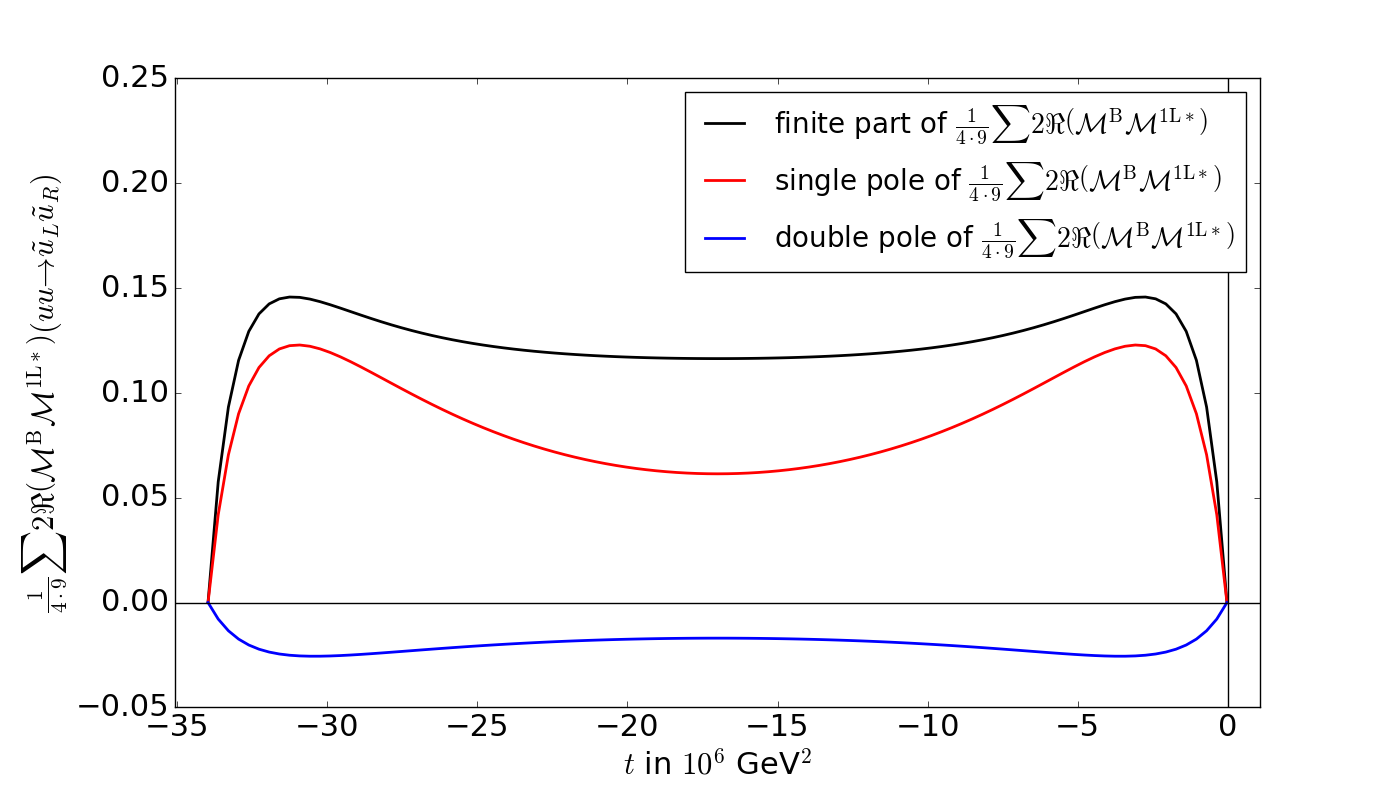
\includegraphics[scale=.5]{figures/MatrixElement_Poles.png}
\caption{Coefficients of $\mathcal{O}(\epsilon^0)$, $\mathcal{O}(\epsilon^{-1})$ and $\mathcal{O}(\epsilon^{-2})$ terms of the dimensionless quantity $\frac{1}{4\cdot 9}\sum 2 \Re (\mathcal{M}^{\mathrm{B}}\mathcal{M}^{\mathrm{1L}})$ of $uu \to \tilde{u}_L\tilde{u}_R$ in the MRSSM as a function of the Mandelstam variable $t$. Final state helicities and colors are averaged. The parameters are fixed to $m_{\tilde{q}} = \mu_R = \unit[1000]{GeV}$, $m_{\tilde{g}} = \unit[2000]{GeV}$, $m_{\sigma} = \unit[5000]{GeV}$ and $\sqrt{s} = \unit[6000]{GeV}$ which is the partonic center-of-mass energy.}\label{fig:MatrixElementPoles}
\end{center}
\end{figure}\\
Note, that the extraction of the single pole does not only involve setting the option \texttt{SetLamda} $\to-1$ and \texttt{Dminus4}$\to 0$, but also setting \texttt{SetLamda}$\to -2$ and \texttt{Dminus4} $\to -2$ and subtracting the term obtained by \texttt{SetLamda}$\to-2$ and \texttt{Dminus4} $\to 0$. In doing so, one accounts for the contraction of double poles with terms of $\mathcal{\epsilon}$. The same applies to the extraction of finite terms. This is summarized schematically in table \ref{tab:poles}.

\begin{table}[!htpb]
\begin{center}
\begin{tabular}{c?c?c}
$\epsilon^i$ & Contribution & Settings in \texttt{FormCalc}\\
\hlinewd{2pt}
$\epsilon^{-2}$ & $\epsilon^{-2}$ & (\texttt{SetLambda} $\to -2$, \texttt{Dminus4} $\to 0$) \\
\hline
$\epsilon^{-1}$ & $\epsilon^{-1}$ & (\texttt{SetLambda} $\to -1$, \texttt{Dminus4} $\to 0$) \\
  & $+\mathcal{O}(\epsilon)\cdot\epsilon^{-1}$ & $+$(\texttt{SetLambda} $\to -2$, \texttt{Dminus4} $\to -2$) \\
  & & $-$(\texttt{SetLambda} $\to -2$, \texttt{Dminus4} $\to 0$)\\
\hline
$\epsilon^{0}$ & $\epsilon^{0}$ & (\texttt{SetLambda} $\to 0$, \texttt{Dminus4} $\to 0$) \\
  & $+\mathcal{O}(\epsilon)\cdot\epsilon^{-1}$ & $+$(\texttt{SetLambda} $\to -1$, \texttt{Dminus4} $\to -2$) \\
  & & $-$(\texttt{SetLambda} $\to -1$, \texttt{Dminus4} $\to 0$)
\end{tabular}
\caption{The table shows what settings need to be adjusted in \texttt{FormCalc} to extract double and single poles as well as finite terms of an expression in \texttt{Mathematica} which contains loop-integrals.}\label{tab:poles}
\end{center}
\end{table}

Now it becomes clear, why the parameter \texttt{FiniteGs} has been introduced. As \texttt{SetLambda} only replaces the loop integrals but not every other term in an expression with the corresponding prefactor of $\epsilon^i$, \texttt{FiniteGs} needs to be set to zero when \texttt{SetLambda} is set to $-1$ or $-2$ and \texttt{FiniteGs}$\to 1$ when \texttt{SetLambda}$\to 0$.\\
The upper plot in figure \ref{fig:MatrixElement} shows the finite contributions from loop diagrams with different topology to $\frac{1}{4\cdot 9}\sum 2 \Re (\mathcal{M}^{\mathrm{B}}\mathcal{M}^{\mathrm{1L}})$ as well as their sum as a function of the Mandelstam variable $t$ where $\frac{1}{4\cdot 9}$ is the averaging over final state spins and colors. The lower plot displays the tree-level absolute squared matrix amplitude with leading order $\alpha_s$ which is compared to its analogue with next-to-leading order $\alpha_s$ and the virtual correction $\frac{1}{4\cdot 9}\sum 2 \Re (\mathcal{M}^{\mathrm{B}}\mathcal{M}^{\mathrm{1L}})$. The latter is not given analytically. It can be seen that the virtual corrections are relatively constant. Referring to eq. \eqref{eq:t}, this suggests that in this case, virtual corrections do enhance the differential cross section in all directions of the beam axis relatively uniformly.
\begin{figure}[!htpb]
\begin{center}
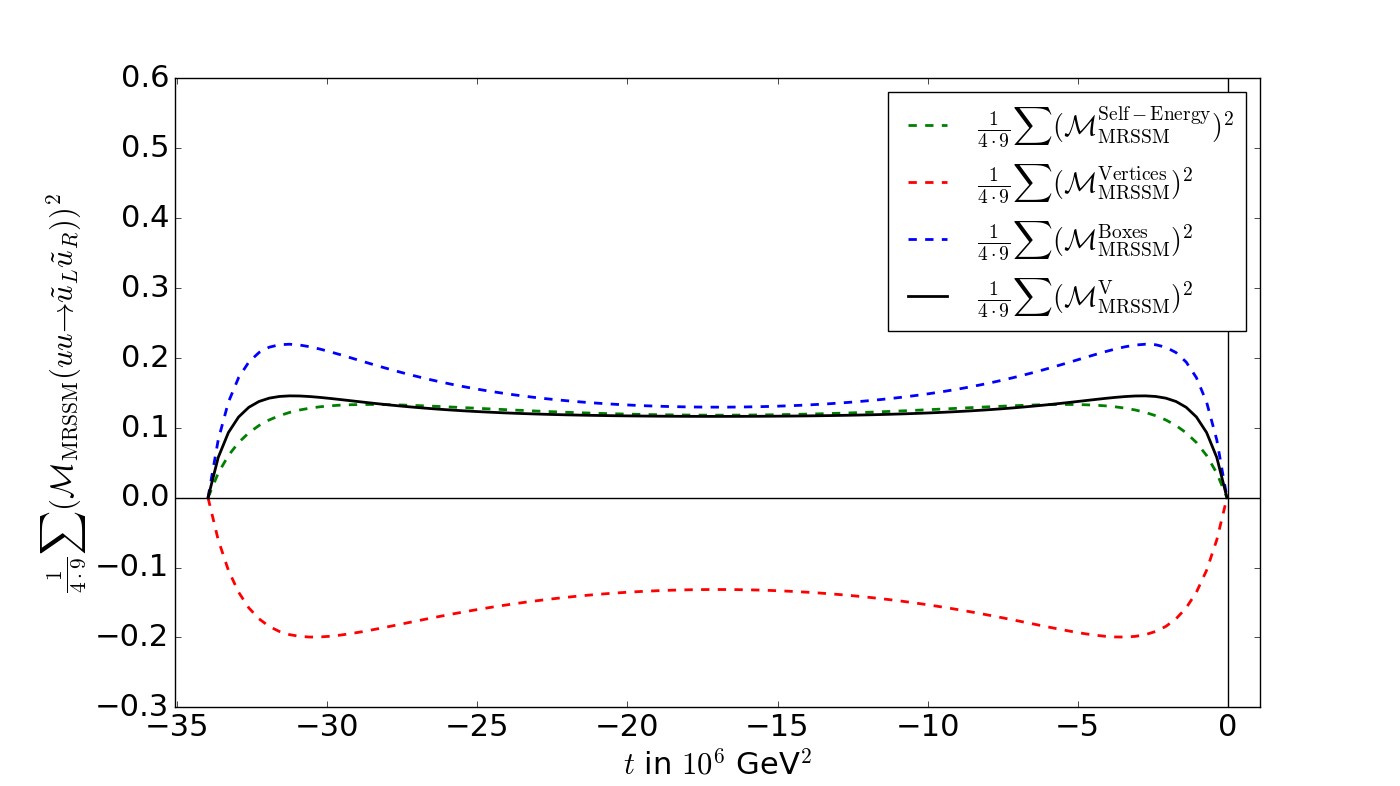
\includegraphics[scale=.5]{figures/MatrixElement_SE_Vertices_Boxes}
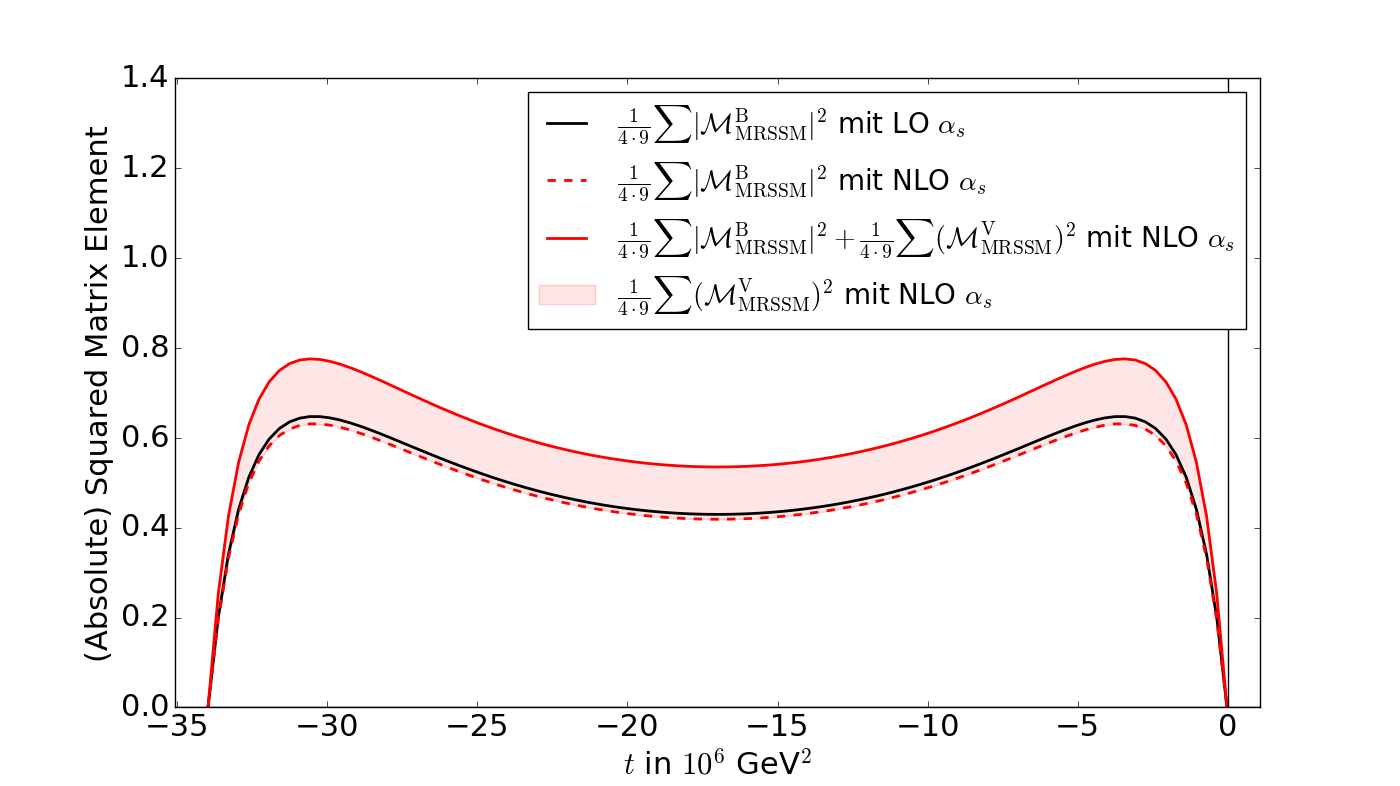
\includegraphics[scale=.5]{figures/MatrixElement.png}
\caption{The figure at the bottom shows the absolute squared matrix element of $uu \to \tilde{u}_L\tilde{u}_R$ in the MRSSM at tree-level with $\alpha_s = 0.135$ from the leading order parton density function $\mathtt{MMHT2014}$\cite{Harland-Lang:2014zoa}, and $\alpha_s = 0.12$ from the next-to-leading order parton density function as well as the contribution from the virtual absolute squared matrix element.\newline 
The figure at the top shows the different contributions and their sum to the virtual corrections. The used parameters are given under fig. \ref{fig:MatrixElementPoles}.}\label{fig:MatrixElement}
\end{center}
\end{figure}